\documentclass[11pt,a4paper]{article}

\usepackage[a4paper,margin=25mm,headheight=15pt]{geometry}
\usepackage{microtype}
\usepackage{amsmath,amssymb,mathtools}
\usepackage{booktabs,array,longtable,multirow,tabularx}
\usepackage{graphicx}
\usepackage[dvipsnames,table]{xcolor}
\usepackage{enumitem}
\usepackage{caption,subcaption}
\usepackage{fancyhdr}
\usepackage{listings}
\usepackage{tikz}
\usetikzlibrary{
  arrows.meta,
  backgrounds,
  calc,
  fit,
  matrix,
  positioning,
  shapes.geometric
}
\usepackage{natbib}
\usepackage{hyperref}
\usepackage[nameinlink,capitalise,noabbrev]{cleveref}
\usepackage{xspace}

\definecolor{AlucluNavy}{HTML}{172A46}
\definecolor{AlucluBlue}{HTML}{246BCE}
\definecolor{AlucluCyan}{HTML}{12A8A8}
\definecolor{AlucluGold}{HTML}{D59A24}
\definecolor{AlucluRed}{HTML}{B64242}
\definecolor{AlucluLight}{HTML}{F2F6FA}
\definecolor{AlucluGray}{HTML}{5C6773}
\definecolor{CodeBackground}{HTML}{F7F8FA}

\hypersetup{
  colorlinks=true,
  linkcolor=AlucluBlue,
  citecolor=AlucluCyan,
  urlcolor=AlucluBlue,
  pdftitle={ALUCLU: A Bounded Multi-Lane Streaming Memory Architecture},
  pdfauthor={Kaan Kadir Aluçlu},
  pdfsubject={Bounded-state recurrent language-model memory},
  pdfkeywords={ALUCLU, recurrent language model, bounded state, linear attention,
    episodic memory, exact cache, long context}
}

\pagestyle{fancy}
\fancyhf{}
\fancyhead[L]{\small\textsc{ALUCLU Technical Paper}}
\fancyhead[R]{\small Kaan Kadir Aluçlu}
\fancyfoot[C]{\thepage}

\setcounter{secnumdepth}{3}
\setcounter{tocdepth}{2}
\setlist{nosep,leftmargin=*}
\captionsetup{font=small,labelfont=bf}
\renewcommand{\arraystretch}{1.16}
\emergencystretch=2em

\lstset{
  backgroundcolor=\color{CodeBackground},
  basicstyle=\ttfamily\small,
  breaklines=true,
  columns=fullflexible,
  frame=single,
  framerule=0.3pt,
  rulecolor=\color{AlucluGray},
  keywordstyle=\color{AlucluBlue}\bfseries,
  commentstyle=\color{AlucluGray}\itshape,
  stringstyle=\color{AlucluCyan},
  showstringspaces=false,
  tabsize=2
}

\newtheorem{definition}{Definition}
\newtheorem{proposition}{Proposition}
\newtheorem{corollary}{Corollary}
\newtheorem{remark}{Remark}

\newcommand{\ALUCLU}{\textsc{Aluclu}\xspace}
\newcommand{\R}{\mathbb{R}}
\newcommand{\E}{\mathbb{E}}
\newcommand{\norm}[1]{\left\lVert #1\right\rVert}
\newcommand{\abs}[1]{\left\lvert #1\right\rvert}
\newcommand{\diag}{\operatorname{diag}}
\newcommand{\softmax}{\operatorname{softmax}}
\newcommand{\softplus}{\operatorname{softplus}}
\newcommand{\sigmoid}{\operatorname{sigmoid}}
\newcommand{\RMSNorm}{\operatorname{RMSNorm}}
\newcommand{\SiLU}{\operatorname{SiLU}}
\newcommand{\LtwoNorm}{\operatorname{L2Normalize}}
\newcommand{\stopgrad}{\operatorname{stopgrad}}
\newcommand{\rank}{\operatorname{rank}}
\newcommand{\median}{\operatorname{median}}
\newcommand{\clip}{\operatorname{clip}}
\newcommand{\state}{\mathcal{S}}
\newcommand{\bigO}{\mathcal{O}}

\title{
  \vspace{-1.2cm}
  {\color{AlucluNavy}\bfseries
  ALUCLU: A Bounded Multi-Lane Streaming Memory Architecture}\\[0.35em]
  \large Adaptive Layered Unified Context with Learned Updates
}
\author{Kaan Kadir Aluçlu\\
\small Independent Researcher and Software Engineer\\
\small \href{https://github.com/kaannsaydamm/ALUCLU}{github.com/kaannsaydamm/ALUCLU}}
\date{Version 0.1.0 -- 30 July 2026}

\begin{document}

\maketitle

\begin{abstract}
\ALUCLU is a decoder-only research architecture for causal sequence modeling
that places four physically different, explicitly bounded memory lanes inside
a single residual block: a dense recurrent fast-weight lane based on a
Gated Delta Rule-2 update, exact sliding-window softmax attention, a
fixed-capacity residual-surprise exact key-value cache, and a segmented
episodic lane with exact recent factors and low-rank archived capsules.
All active branches read the same normalized token representation and are
combined by learned token-wise mixture coefficients before a SwiGLU
feed-forward stage. The design is motivated by a simple systems observation:
recency, dense statistical continuity, sparse exceptional events, and
compressed temporal episodes impose different storage and access
requirements, so forcing all four into one state representation creates
avoidable trade-offs.

This paper specifies the implemented recurrence, cache replacement policy,
episodic life cycle, mass-conserving router, thin-QR small-core SVD
compression, persistent-state accounting, and causal execution semantics. It
also states what the current evidence does and does not establish. The
reference implementation is a portable token-recurrent correctness backend,
not a fused accelerator kernel and not a trained frontier model. Fifty
automated tests validate causality, scan/step equivalence in evaluation mode,
bounded state, compression error accounting, priority retention, routing mass
conservation, and finite gradients on small cases. A deliberately small CPU
learnability diagnostic reaches \(90.43\%\) answer accuracy on its own MQAR
protocol, while a saturated-state CPU benchmark reports a median recurrent
decode rate of \(143.71\) tokens/s for a \(363{,}385\)-parameter configuration.
These measurements demonstrate executable mechanics and reproducible
instrumentation only; broad quality or speed superiority requires the
larger controlled evaluation program defined here.
\end{abstract}

\begin{center}
\begin{minipage}{0.94\textwidth}
\small
\textbf{Türkçe özet.}
\ALUCLU, nedensel dizi modelleme için dört farklı ve açıkça sınırlı bellek
yolunu aynı residual blokta birleştiren decoder-only bir araştırma
mimarisidir: Gated Delta Rule-2 tabanlı yoğun recurrent fast-weight belleği,
sabit pencereli exact softmax attention, sabit kapasiteli residual-surprise
exact key-value cache ve yakın geçmişi exact factor, eski bölümleri düşük
ranklı kapsül olarak tutan episodic bellek. Yollar aynı normalize edilmiş token
temsilini okur ve SwiGLU katmanından önce token bazında öğrenilen katsayılarla
birleştirilir. Makale, çalışan referans kodun denklemlerini, nedensellik
sırasını, state ve hesap maliyetini, sıkıştırma hata defterini, bilinen
başarısızlık kiplerini ve adil deney protokolünü ayrıntılı biçimde verir.
Mevcut sonuçlar bir dünya rekoru veya SOTA iddiası değildir; uygulamanın
çalıştığını, sınırlarının ölçülebildiğini ve daha büyük deneylere hazır bir
doğruluk oracle'ı sunduğunu gösterir.
\end{minipage}
\end{center}

\vspace{0.5em}
\noindent\textbf{Keywords:}
bounded-state sequence modeling; recurrent language models; linear attention;
associative memory; exact cache; episodic compression; long-context evaluation.

\clearpage
\tableofcontents
\clearpage

\section{Introduction}
\label{sec:introduction}

Long-context sequence modeling is constrained by three resources that cannot
be optimized independently: representational capacity, memory traffic, and
arithmetic work. Full causal self-attention preserves direct token-to-token
access, but its key-value state grows with the processed sequence and its
prefill attention matrix grows quadratically without additional structure.
Recurrent and linear-attention models replace that growing state with a
fixed-size summary, but any finite summary must eventually merge, overwrite,
or discard independent information. Sparse caches preserve selected records
exactly, yet a selection rule can retain the wrong records. Compressed
episodic representations extend the age horizon, but compression creates a
measurable approximation error.

\ALUCLU starts from the premise that these are not four implementations of one
memory abstraction. They are four different physical memory regimes:

\begin{table}[h]
\centering
\caption{The four memory regimes used by \ALUCLU. ``Exact'' is local to the
stored representation and never means unbounded exact recall.}
\label{tab:memory-regimes}
\begin{tabularx}{\textwidth}{@{}p{0.18\textwidth}p{0.21\textwidth}
  p{0.23\textwidth}X@{}}
\toprule
Regime & Primary role & Physical budget & Principal failure mode \\
\midrule
Dense recurrence & Continuous global statistics & Fixed fast-weight matrix
per layer & Interference and decay \\
Local softmax & Precise recent interactions & Last \(W\) projected keys and
values & Hard recency horizon \\
Surprise cache & Sparse exceptional records & Highest-priority \(C_x\)
projected KV records & Selection mismatch and cache freezing \\
Episodic capsules & Longer temporal organization & Current segment, \(K\)
live segments, \(C\) rank-\(r\) archive capsules & Compression and overwrite \\
\bottomrule
\end{tabularx}
\end{table}

The architecture places these regimes in parallel inside selected transformer-
like residual blocks. Every layer has a Gated Delta Rule-2 recurrent lane.
Local, exact-cache, and episodic lanes are scheduled at configurable layer
intervals. They all consume the same normalized token representation rather
than forming a serial chain. Their outputs are independently normalized and
combined with learned token-wise coefficients. This arrangement gives the
model an explicit choice between a dense recurrent estimate, exact recent
evidence, a sparse set of high-write-residual events, and temporally segmented
compressed evidence.

\subsection{Design question}

The project asks a deliberately narrower and more testable question than
``What is the universally best language-model architecture?'':

\begin{quote}
Can one build an executable causal reference architecture whose persistent
decode state is bounded by configuration, whose heterogeneous memory losses
are visible in state and metrics, and whose interfaces permit exact
token-by-token auditing before specialized kernels or large-scale training?
\end{quote}

This question matters because algorithmic asymptotics alone do not determine
real performance. A theoretically constant-state recurrence can be slower than
optimized attention if implemented as a Python token loop. A low-rank archive
can have a long nominal horizon but poor task recall. A small cache can be
``exact'' for accepted keys while missing the one key a future query needs.
Consequently, \ALUCLU treats equations, code semantics, state bytes, benchmark
protocols, and claim boundaries as parts of one engineering object.

\subsection{Contributions}

The present release makes the following concrete contributions.

\begin{enumerate}
  \item It specifies and implements a four-lane decoder block with explicit
  scan, chunk, and recurrent-step interfaces and immutable external state
  containers.

  \item It couples a Gated Delta Rule-2 write residual to a fixed-capacity
  exact KV cache. The cache retains the highest observed scalar residual
  priorities under a deterministic strict-replacement policy.

  \item It implements a bounded episodic hierarchy with exact current/live
  factor sums, low-rank archive capsules, exact positive denominator
  statistics, a TensorSketch-assisted router, and a Frobenius error ledger.

  \item It derives the persistent payload, retained temporal budget, and
  token-cost terms from the actual state fields instead of using an informal
  ``constant memory'' label.

  \item It provides a mass-normalized routing construction that preserves the
  unweighted denominator mass in exact arithmetic when numerical safety
  clamps are inactive, while making the clamp qualification explicit.

  \item It supplies an MIT-licensed Python package, command-line tools,
  protocol manifests, multilingual documentation, reproducible JSON evidence,
  and an automated release gate with 50 tests.

  \item It defines a staged evaluation program that separates small
  correctness and learnability diagnostics from model-quality, accelerator,
  energy, and long-context claims.
\end{enumerate}

\subsection{Evidence contract}
\label{sec:evidence-contract-intro}

The strongest conclusions supported by the current artifact are mechanical:
the code executes, its configured state is bounded, tested causal paths agree
between full scans and recurrent stepping in evaluation mode, and the recorded
small CPU experiments are reproducible under their declared protocols. The
artifact does \emph{not} establish frontier language-model quality, universal
speed superiority, an optimal memory allocation, or a production GPU kernel.

We use three labels throughout the paper:

\begin{description}
  \item[Implemented] The behavior exists in the released source code and is
  connected to the public model path.
  \item[Measured] A result file records the protocol, configuration,
  environment, and numerical outcome.
  \item[Proposed] The experiment or optimization is fully specified but has
  not been executed as evidence for this release.
\end{description}

This vocabulary is intentionally conservative. It prevents a common category
error in architecture research: presenting a promising mechanism, a Python
prototype, or an asymptotic argument as though it were already an end-to-end
systems result.

\subsection{Paper organization}

\Cref{sec:related-work} positions the design among recurrent, attention,
hybrid, and long-context evaluation work. \Cref{sec:problem-contract} defines
the causal interface and measurable Pareto contract. \Cref{sec:architecture}
describes the block and execution order. \Cref{sec:memory-lanes} gives the
implemented equations, while \Cref{sec:theory} derives state, complexity, and
error properties. \Cref{sec:implementation} maps the specification to code.
\Cref{sec:evaluation,sec:results} separate the planned evaluation matrix from
the measurements already available. \Cref{sec:limitations} lists failure
modes and physical limits. The appendices provide configuration, state, test,
and reproduction details.

\section{Related Work}
\label{sec:related-work}

\subsection{Linear attention and fast-weight memory}

Kernelized linear attention rewrites causal attention as a recurrent
accumulation of key-value statistics, replacing a context-length-dependent KV
cache with a state whose size is fixed once feature and value dimensions are
fixed \citep{katharopoulos2020transformers}. This view exposes both the appeal
and the limitation of the method: decode state stops growing, but many
associations must share one finite matrix. \citet{schlag2021linear} interpreted
the matrix as fast weights and introduced a delta update that reads the value
currently associated with a key and writes a residual rather than adding an
unconditional outer product.

DeltaNet made this update practical at language-model scale through a
chunkwise sequence-parallel algorithm and studied mixtures with
sliding-window or sparse global attention \citep{yang2024parallelizing}. Gated
Delta Networks combined targeted correction with adaptive forgetting
\citep{yang2025gated}. The Gated DeltaNet-2 technical report further separates
channel-wise erase and write gates while retaining adaptive channel decay
\citep{hatamizadeh2026gated}. Because the last work is a 2026 preprint, its
architectural and empirical findings are attributed to its authors rather than
treated as independently established.

\ALUCLU uses an independently written token-recurrent update in this
erase/write-separated design class. It is not a reproduction of the official
chunkwise kernel and its CPU measurements do not inherit any reported
accelerator performance.

\subsection{Selective state-space models}

Mamba demonstrated that input-dependent selective state-space parameters can
provide content-sensitive sequence processing with a fixed recurrent state and
a hardware-aware training form \citep{gu2024mamba}. Structured State Space
Duality connected semiseparable state-space operators to attention-like
matrices and led to Mamba-2 \citep{dao2024transformers}. Mamba-3 extends this
line with richer discretization, complex-valued dynamics, and SISO/MIMO
formulations; the current official record identifies it as an ICLR 2026 oral
paper \citep{lahoti2026mamba3}.

These models are essential bounded-state comparators, but \ALUCLU makes a
different decomposition. Its recurrent lane is a matrix-valued delta memory;
exact recent context, selected exact records, and segmented compressed history
remain explicit separate states. State-space dualities may inform
kernelization and comparisons, but do not make the four lanes algebraically
equivalent to Mamba-family layers.

\subsection{Recall limits and local/global hybrids}

Zoology introduced MQAR and showed that associative recall explains a
substantial part of the gap observed between attention and efficient
gated/convolutional models in its experiments \citep{arora2024zoology}. Based
framed a recurrent-state-size/recall trade-off and combined linear attention
with exact sliding-window attention, supported by IO-aware kernels
\citep{arora2024based}. These results motivate \ALUCLU's exact local lane:
recent interactions retain direct softmax access while the recurrent lane
spends fixed state on compressed global structure.

Recent hybrids allocate memory differently. Kimi Linear combines a
fine-grained delta recurrence with Multi-Head Latent Attention layers
\citep{kimiteam2025kimi}; because those attention layers retain a growing
cache, the whole hybrid does not satisfy \ALUCLU's strict saturated-state
contract. Native Hybrid Attention places recurrent long-term KV slots and
recent sliding-window tokens in a shared softmax read
\citep{du2026native}. Infini-attention combines masked local attention with a
bounded compressive memory \citep{munkhdalai2024infini}. \ALUCLU instead keeps
four reads semantically separate, normalizes them separately, and mixes their
outputs. This avoids treating a positive-linear denominator as a softmax
partition function and makes every lane independently ablatable.

\subsection{Residual-selected exact memory}

HOLA provides the closest direct precedent for an exact complement to delta
memory: it retains a bounded set of KV pairs whose writes have large residual
relative to the compressive state \citep{cui2026hippocampus}. \ALUCLU's cache
is motivated by the same high-level idea but defines its own policy. It uses
the RMS of its Gated Delta Rule-2 write residual, detaches the scalar priority,
applies deterministic strict top-capacity admission, and reads retained
projected KV pairs with exact softmax. ``Exact'' therefore describes the
attention over retained records, not the selection of arbitrary history. HOLA
is a recent single-author preprint, so comparative conclusions require a
matched replication.

Growing and sparse memories clarify the fixed-state boundary. Memory Caching
stores recurrent checkpoints, so its usable memory grows with the sequence
\citep{behrouz2026memory}. Sparse Delta Memory spends a fixed but much larger
state on sparse explicit addressing \citep{cabannes2026sparse}. Both are useful
controls: one tests the benefit of relaxing bounded state; the other tests a
different allocation of a fixed state budget.

\subsection{Exact attention systems}

FlashAttention computes exact softmax attention with IO-aware tiling, reducing
high-bandwidth memory traffic without changing attention semantics
\citep{dao2022flashattention}. FlashAttention-2 improves work partitioning and
parallelism \citep{dao2024flashattention2}. These works define the systems
standard for implementing \ALUCLU's local and cache reads, but address a
different axis from architectural state growth. An IO-efficient full-attention
kernel still carries context-dependent KV state, while an asymptotically
bounded recurrence can still be slow if implemented as a Python token loop.

\subsection{Bounded low-rank compression}

\ALUCLU's episodic lane keeps current and recent segments as exact factor sums
for a positive linear-attention numerator, then merges older segments into a
finite ring of rank-bounded capsules. Householder triangularization supplies
the numerical basis for thin QR \citep{householder1958unitary}. The SVD of the
resulting small core represents the same factor product before truncation, and
the Eckart--Young result characterizes the retained best-rank approximation
for the local matrix \citep{eckart1936approximation}. Thin-SVD modification
methods provide a streaming numerical precedent \citep{brand2006fast};
Frequent Directions is a principled deterministic alternative with different
covariance guarantees \citep{ghashami2016frequent}.

This background supports a narrow claim: the discarded singular tail is an
algebraic Frobenius error for the matrix being compressed. It is not a bound on
task loss or arbitrary recall. \ALUCLU keeps the positive denominator summary
outside the truncated factors and records a conservative cumulative error
ledger. When the finite ring wraps, overwritten history is unavailable.

\subsection{Sketch-based routing}

TensorSketch gives an explicit randomized feature map for polynomial kernels
through compressed tensor-product features
\citep{pham2013fast}. PolySketchFormer demonstrates polynomial sketching in
causal sequence models \citep{kacham2024polysketchformer}. \ALUCLU uses the
method more narrowly: it estimates polynomial similarity only among a finite
set of current/live/archive slots, alongside a degree-one route.

A 2025 TensorSketch manuscript explicitly corrects the variance bound
associated with the original account \citep{pham2025tensor}; consequently this
paper does not repeat the earlier variance expression. Finite sketch width and
replica count create routing error. Sketching neither reconstructs
rank-truncated numerator information nor recovers an overwritten capsule.

\subsection{Capacity and long-context evaluation}

Task-specific separations show that some lookup problems require recurrent
state growing linearly with input size even where relatively small
Transformers suffice \citep{bhattamishra2024separations}. These results do not
directly prove a task-accuracy bound for \ALUCLU, but they reinforce the need
for an honest finite-capacity contract.

Evaluation must also extend beyond one synthetic needle. RULER adds
multi-needle retrieval, multi-hop tracing, and aggregation across controlled
lengths \citep{hsieh2024ruler}. NoLiMa removes easy literal overlap between
questions and evidence \citep{modarressi2025nolima}. BABILong distributes
facts required for multi-step reasoning through long natural-text distractors
\citep{kuratov2024babilong}. HELMET shows why synthetic retrieval alone cannot
stand in for diverse application-centric long-context performance
\citep{yen2025helmet}. \ALUCLU evaluation should therefore report length and
capacity curves for synthetic recall together with language-model loss and
application-oriented task categories.

\subsection{Positioning}

Prior work supports three premises, not an \ALUCLU performance conclusion.
First, recurrent delta and state-space mechanisms provide bounded global state
but face finite-capacity interference. Second, exact local or selected memory
can complement a compressive state at an explicit cost in bytes and reads.
Third, low-rank and sketching methods make compression measurable but cannot
defeat information limits. \ALUCLU's contribution is the particular bounded
four-lane allocation, its independently testable execution semantics, and its
claim-and-measurement contract. Whether that composition improves a
quality--latency--traffic--energy Pareto frontier remains an empirical
question.

\section{Problem Formulation and Claim Contract}
\label{sec:problem-contract}

\subsection{Causal streaming interface}

Let \(x_{1:T}\) be a token sequence and let \(f_\theta\) be a decoder-only
model. At token \(t\), the recurrent interface computes
\begin{equation}
  (y_t,\state_t)=f_\theta(x_t,\state_{t-1}),
  \label{eq:stream-interface}
\end{equation}
where \(y_t\) denotes logits or a hidden representation and \(\state_t\) is
the complete persistent state. Causality requires that \(y_t\) and
\(\state_t\) be functions only of \(x_{1:t}\). For a fixed configuration
\(\mathcal{C}\), bounded persistent state means that there exists a finite
quantity \(M(\mathcal{C},B)\) such that
\begin{equation}
  \operatorname{bytes}(\state_t)\le M(\mathcal{C},B)
  \qquad \text{for every }t,
  \label{eq:bounded-state}
\end{equation}
for batch size \(B\). The bound may depend on width, layers, cache capacities,
window size, ranks, data types, and batch size, but not on the number of
already processed tokens.

Equation~\eqref{eq:bounded-state} concerns inference payload. It does not imply
that training activation memory is independent of \(T\): a naive autograd
scan retains a graph whose size grows with the number of untruncated steps.
Likewise, bounded logical tensor payload does not imply bounded allocator
workspace or constant wall-clock latency at archive compression boundaries.

\subsection{Inclusive write-then-read semantics}

The implemented memory lanes use inclusive causal semantics. At time \(t\),
the current token is first admitted to, or used to update, the relevant state;
the read then uses that updated state. Symbolically,
\begin{equation}
  \state_t=\operatorname{write}(x_t,\state_{t-1}),\qquad
  y_t=\operatorname{read}(x_t,\state_t).
  \label{eq:write-read}
\end{equation}
For language modeling, loss is computed between
\(\mathrm{logits}_{1:T-1}\) and labels \(x_{2:T}\), so inclusive internal
memory is compatible with next-token prediction. The ordering is important at
local-window boundaries, exact-cache replacement events, and episodic segment
seals; a read-before-write implementation would define a different model.

\subsection{Pareto objective}

No single scalar called ``performance'' captures the intended design target.
For model and hardware configuration \(\mathcal{C}\), define
\begin{equation}
  \mathbf{J}(\mathcal{C}) =
  \left(
  Q_{\mathrm{task}},
  R_{\mathrm{recall}},
  \tau_{\mathrm{prefill}},
  \tau_{\mathrm{decode}},
  M_{\mathrm{peak}},
  M_{\mathrm{state}},
  E_{\mathrm{token}}
  \right),
  \label{eq:pareto-vector}
\end{equation}
where \(Q_{\mathrm{task}}\) is downstream quality,
\(R_{\mathrm{recall}}\) is controlled retrieval accuracy,
\(\tau_{\mathrm{prefill}}\) and \(\tau_{\mathrm{decode}}\) are throughput,
\(M_{\mathrm{peak}}\) is peak runtime memory, \(M_{\mathrm{state}}\) is
persistent state payload, and \(E_{\mathrm{token}}\) is energy per generated
token. An architecture is interesting only if it shifts a relevant Pareto
front under matched parameters, tokens, optimizer, precision, compiler,
hardware, and quality constraints.

For this reason, the current release does not optimize
Equation~\eqref{eq:pareto-vector} into one headline score. It exposes the
budgets and protocols needed to measure each coordinate independently.

\subsection{Information-capacity lower bound}

Suppose a finite state contains at most \(Q\) bits and a task asks the model to
recover \(N\) independent values drawn uniformly from an alphabet
\(\mathcal{V}\), with query keys known externally. The values alone have
\(N\log_2\abs{\mathcal{V}}\) bits of entropy. Lossless recovery for all
possible assignments therefore requires
\begin{equation}
  Q\ge N\log_2\abs{\mathcal{V}},
  \qquad\text{or equivalently}\qquad
  N\le \frac{Q}{\log_2\abs{\mathcal{V}}}.
  \label{eq:counting-bound}
\end{equation}
The bound is optimistic: it ignores floating-point noise, query ambiguity,
router collisions, rank constraints, and the computational limits of the
readout. It nevertheless rules out unbounded exact arbitrary recall from a
fixed-precision state. \ALUCLU therefore treats forgetting and approximation
as explicit budgeted operations rather than hiding them behind an unlimited
context-length label.

\subsection{Fair-comparison requirements}
\label{sec:fair-comparison}

An end-to-end comparison is valid only when the following conditions are
reported and, where relevant, matched:

\begin{itemize}
  \item training data, tokenizer, token count, data order, and contamination
  controls;
  \item parameter count, effective depth and width, optimizer, schedule,
  batch tokens, and gradient clipping;
  \item inference precision, quantization, batch size, prompt length,
  generation length, and sampling policy;
  \item software versions, compiler flags, kernel implementation, device,
  power mode, and thermal state;
  \item whether model loading, random-token generation, compilation,
  synchronization, and state allocation occur inside the timed region;
  \item accuracy or loss at the throughput operating point;
  \item median and dispersion across repeated runs, not only a best sample.
\end{itemize}

The portable reference backend is primarily a semantic oracle. It should be
compared with optimized systems only after the same recurrence has a
specialized implementation, and both semantic equality and numerical drift
have been tested against the oracle.

\subsection{Progression gates}

The project uses four evidence gates.

\begin{enumerate}
  \item \textbf{Mechanics gate:} unit invariants, causality, scan/step
  equivalence, state saturation, serialization policy, and finite gradients.
  \item \textbf{Learnability gate:} multiple seeds and controlled synthetic
  tasks, including MQAR protocols whose target alignment is frozen.
  \item \textbf{Quality gate:} matched-token pretraining and long-context
  downstream evaluation against serious recurrent, attention, and hybrid
  baselines.
  \item \textbf{Systems gate:} fused kernels, profiler evidence, peak memory,
  decode and prefill throughput, energy, and quality-matched comparisons on
  target accelerators.
\end{enumerate}

The present v0.1.0 artifact passes the mechanics gate for its tested domain and
contains one small learnability diagnostic. The larger quality and systems
gates remain proposed work.

\section{Architecture}
\label{sec:architecture}

\subsection{Name and structural principle}

\textbf{ALUCLU} expands to \textbf{Adaptive Layered Unified Context with
Learned Updates}. ``Layered'' denotes scheduled placement across depth and the
separation of physical memory regimes. ``Unified context'' denotes a single
token representation assembled from all active lanes. ``Learned updates''
refers both to recurrent write dynamics and token-wise fusion. The name is
written with ASCII \texttt{C} in code, package names, and URLs.

The unit of composition is \texttt{AlucluBlock}. Given input \(x_t^{(\ell)}\),
the block first computes
\begin{equation}
  h_t^{(\ell)}=\RMSNorm_{\mathrm{mix}}\!\left(x_t^{(\ell)}\right).
\end{equation}
Every active memory lane reads \(h_t^{(\ell)}\) in parallel. A lane never
consumes another lane's output as its input. This keeps lane semantics
separable and lets each state transition be audited against the same token.

\subsection{Layer scheduling}

Every one of the \(L\) layers contains a Gated Delta lane. The other lanes are
periodic:
\begin{align}
  N_{\mathrm{local}}
  &=\left\lfloor\frac{L}{e_{\mathrm{local}}}\right\rfloor,\\
  N_{\mathrm{epi}}
  &=\left\lfloor\frac{L}{e_{\mathrm{epi}}}\right\rfloor,\\
  N_{\mathrm{exact}}
  &=\left\lfloor\frac{L}{e_{\mathrm{exact}}}\right\rfloor,
  \label{eq:branch-counts}
\end{align}
when the corresponding configuration exists. Here each \(e\) is the
``every'' interval. This schedule permits a recurrent backbone at every depth
while concentrating higher-state or higher-latency lanes at selected blocks.

\subsection{Block data flow}

\Cref{fig:block} shows the implemented data flow. The residual-surprise cache
receives its scalar insertion priority from the Gated Delta write residual,
but its query, key, and value projections still read \(h_t^{(\ell)}\).

\begin{center}
\resizebox{\textwidth}{!}{%
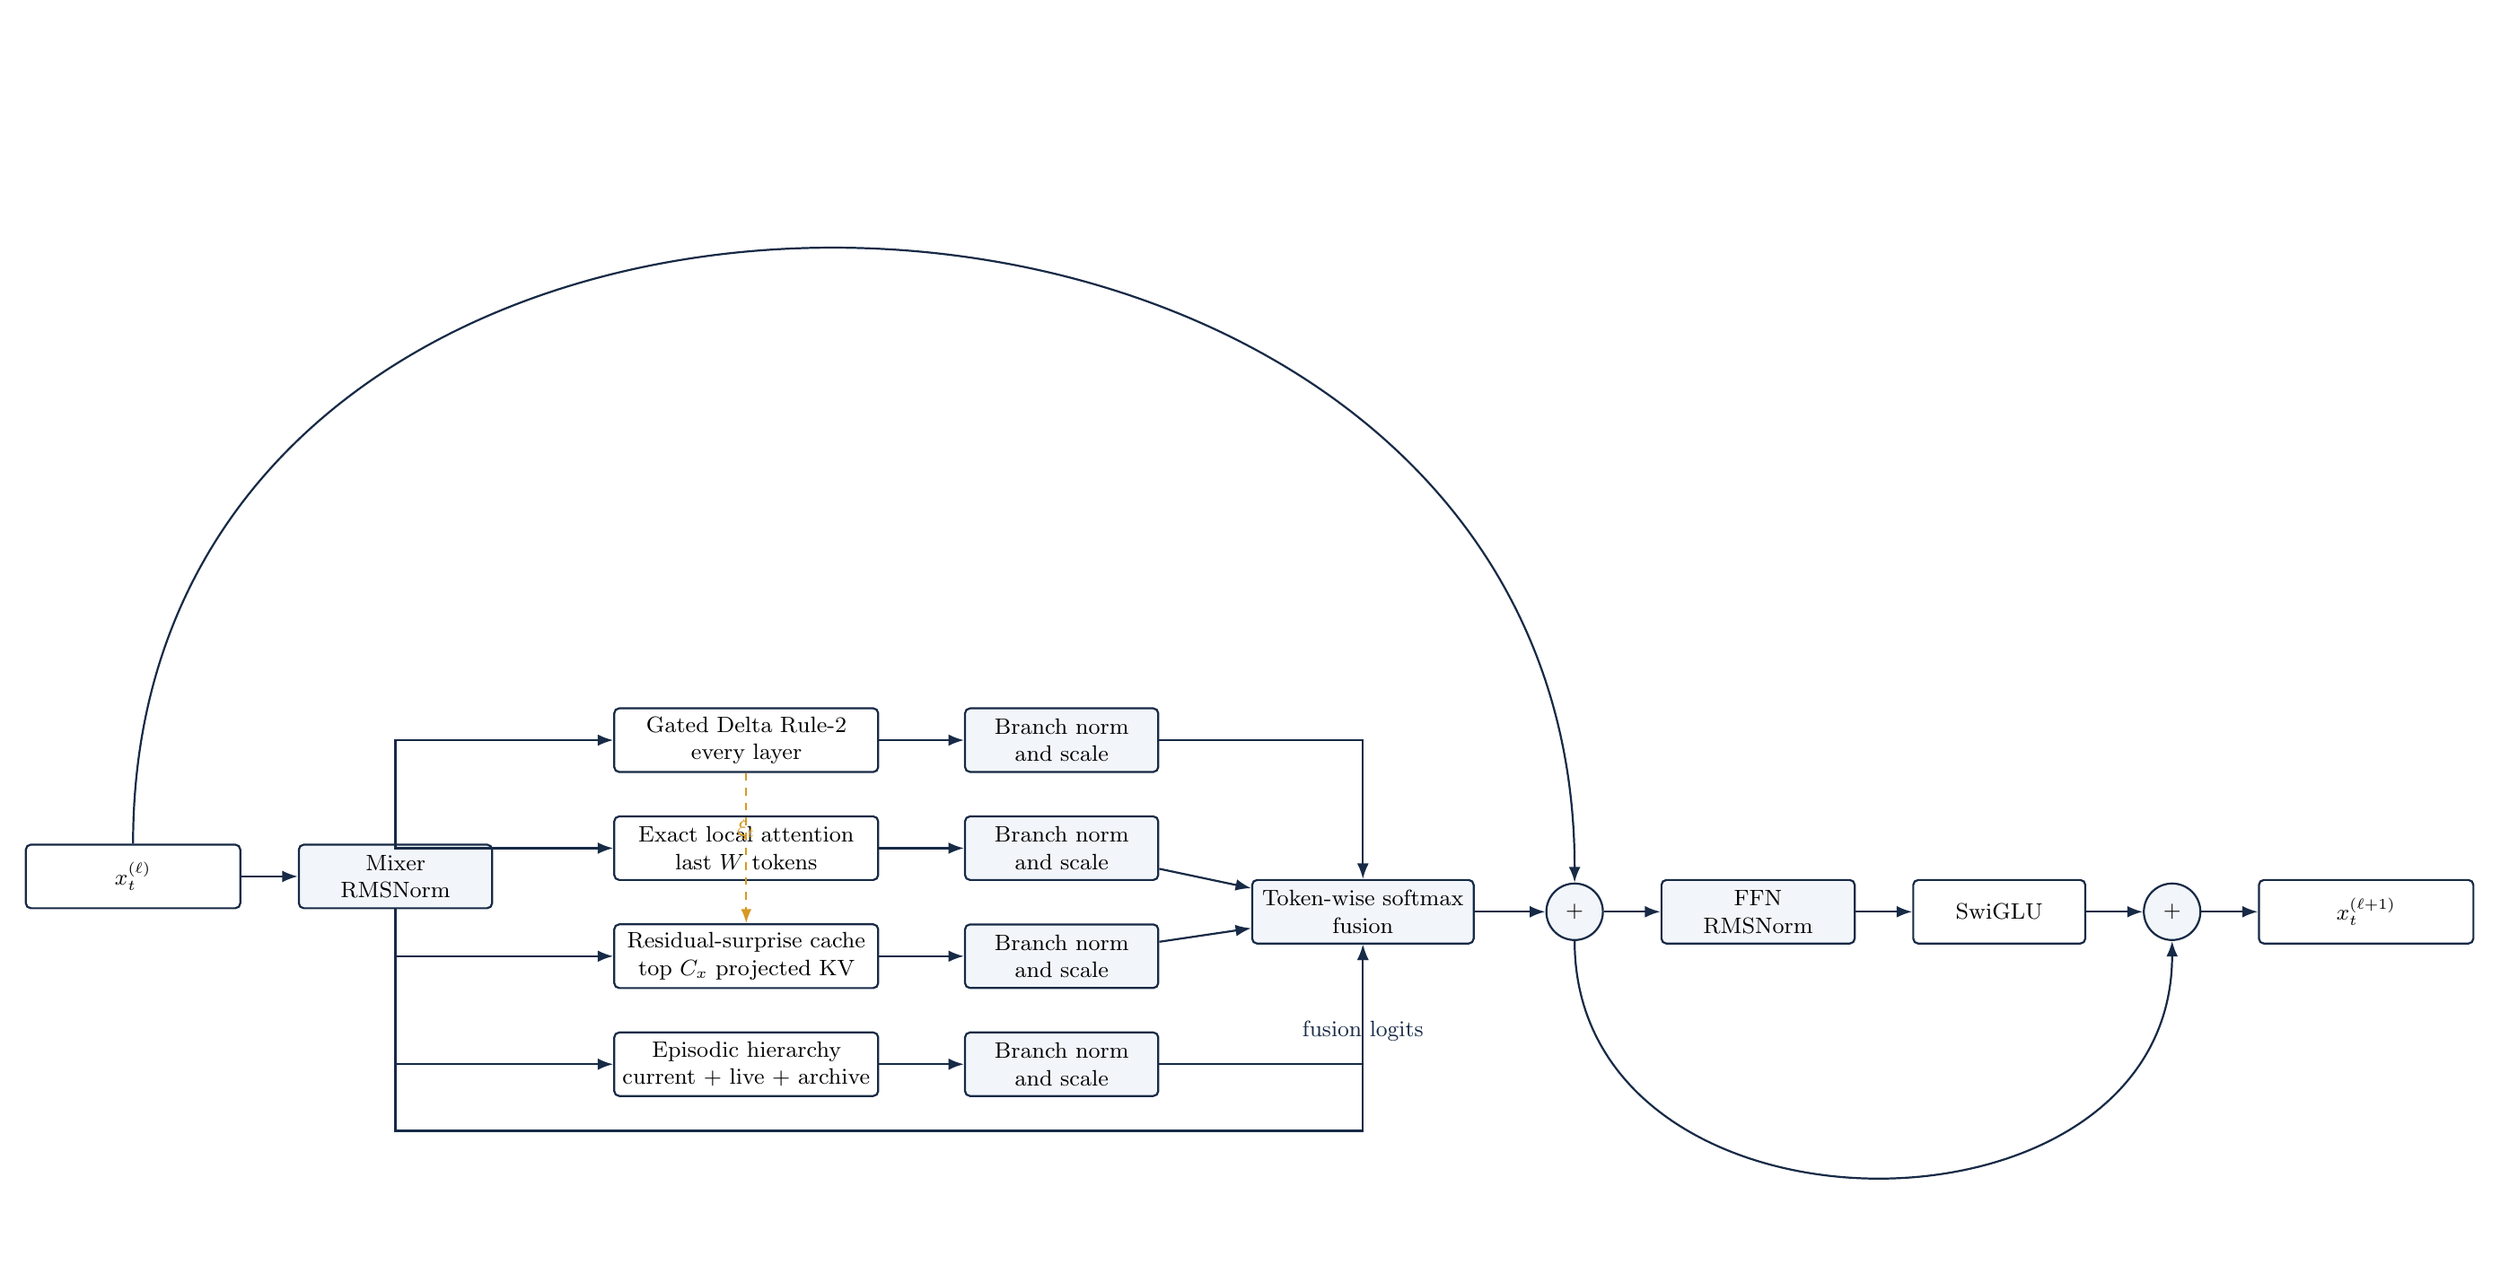
\begin{tikzpicture}[
  node distance=6mm and 8mm,
  every node/.style={font=\small},
  box/.style={draw=AlucluNavy,rounded corners=2pt,thick,fill=white,
    align=center,minimum height=9mm},
  lane/.style={box,text width=35mm},
  norm/.style={box,fill=AlucluLight,text width=25mm},
  sum/.style={circle,draw=AlucluNavy,thick,fill=AlucluLight,
    minimum size=8mm,inner sep=0pt},
  arrow/.style={-{Latex[length=2.2mm]},thick,color=AlucluNavy},
  signal/.style={-{Latex[length=2mm]},dashed,color=AlucluGold,thick}
]
\node[box,text width=28mm] (input) {\(x_t^{(\ell)}\)};
\node[norm,right=of input] (mixnorm) {Mixer\\RMSNorm};

\node[lane,above right=10mm and 17mm of mixnorm] (gdn)
  {Gated Delta Rule-2\\every layer};
\node[lane,below=of gdn] (local)
  {Exact local attention\\last \(W\) tokens};
\node[lane,below=of local] (cache)
  {Residual-surprise cache\\top \(C_x\) projected KV};
\node[lane,below=of cache] (epi)
  {Episodic hierarchy\\current + live + archive};

\node[norm,right=12mm of gdn] (ng) {Branch norm\\and scale};
\node[norm,right=12mm of local] (nl) {Branch norm\\and scale};
\node[norm,right=12mm of cache] (nc) {Branch norm\\and scale};
\node[norm,right=12mm of epi] (ne) {Branch norm\\and scale};

\node[box,fill=AlucluLight,text width=29mm,right=13mm of nl,
  yshift=-9mm] (fusion) {Token-wise softmax\\fusion};
\node[sum,right=10mm of fusion] (add1) {\(+\)};
\node[norm,right=8mm of add1] (ffnnorm) {FFN\\RMSNorm};
\node[box,text width=22mm,right=8mm of ffnnorm] (swiglu) {SwiGLU};
\node[sum,right=8mm of swiglu] (add2) {\(+\)};
\node[box,text width=28mm,right=8mm of add2] (output)
  {\(x_t^{(\ell+1)}\)};

\draw[arrow] (input) -- (mixnorm);
\draw[arrow] (mixnorm) |- (gdn);
\draw[arrow] (mixnorm) |- (local);
\draw[arrow] (mixnorm) |- (cache);
\draw[arrow] (mixnorm) |- (epi);
\draw[signal] (gdn) -- node[above,text=AlucluGold]
  {\(\xi_t\)} (cache);

\draw[arrow] (gdn) -- (ng);
\draw[arrow] (local) -- (nl);
\draw[arrow] (cache) -- (nc);
\draw[arrow] (epi) -- (ne);
\draw[arrow] (ng) -| (fusion);
\draw[arrow] (nl) -- (fusion);
\draw[arrow] (nc) -- (fusion);
\draw[arrow] (ne) -| (fusion);
\draw[arrow] (mixnorm) -- ++(0,-36mm) -| node[pos=0.82,below]
  {fusion logits} (fusion);
\draw[arrow] (fusion) -- (add1);
\draw[arrow] (add1) -- (ffnnorm);
\draw[arrow] (ffnnorm) -- (swiglu);
\draw[arrow] (swiglu) -- (add2);
\draw[arrow] (add2) -- (output);
\draw[arrow] (input) to[out=90,in=90,looseness=1.45] (add1);
\draw[arrow] (add1) to[out=-90,in=-90,looseness=1.35] (add2);
\end{tikzpicture}
}
\captionof{figure}{\ALUCLU block. Solid arrows carry vectors. The dashed arrow carries
the scalar Gated Delta write-surprise signal used by the exact-cache
replacement policy. Every memory lane otherwise reads the same normalized
token.}
\label{fig:block}
\end{center}

\subsection{Streaming causal stems}

The Gated Delta and episodic lanes each begin with an independent causal
depthwise convolution of kernel width \(\kappa\). For an input chunk,
\begin{align}
  c &= [h_{\mathrm{history}};x_{1:T}],\\
  \widetilde h_{1:T} &= \operatorname{DWConv1D}(c),\\
  h_{\mathrm{history}}' &= c_{-(\kappa-1):}.
  \label{eq:stream-conv}
\end{align}
The persistent history has \(B(\kappa-1)d\) elements. Kernels are initialized
to identity by setting all weights to zero except the final causal tap, which
is one, with zero bias. Thus adding the stem does not perturb the initial
token path while allowing training to learn short causal filtering.

\subsection{Token-wise branch fusion}
\label{sec:fusion}

Let \(b_{t,j}\) be active branch \(j\)'s output. Each branch has a separate
normalizer and learned scalar:
\begin{equation}
  \widetilde b_{t,j}
  =s_j\,\RMSNorm_j(b_{t,j}).
\end{equation}
For more than one branch, the mixture is
\begin{align}
  \alpha_t &= \softmax(W_fh_t+b_f),\\
  f_t &= \sum_j\alpha_{t,j}\widetilde b_{t,j},
  \qquad \alpha_{t,j}>0,\quad\sum_j\alpha_{t,j}=1.
  \label{eq:fusion}
\end{align}
The coefficients form a convex combination of the \emph{scaled normalized}
branches. Because \(s_j\) is unconstrained, \(f_t\) is not necessarily in the
convex hull of the raw \(b_{t,j}\). The projection is initialized to zero, so
the initial coefficients are uniform; all branch scales begin at one.

The residual and feed-forward path is
\begin{align}
  x_t' &= x_t+\operatorname{Dropout}(f_t),\\
  (g_t,v_t) &=
  \operatorname{split}\!\left(W_{\mathrm{in}}\RMSNorm(x_t')\right),\\
  u_t &= W_{\mathrm{out}}\!\left(\SiLU(g_t)\odot v_t\right),\\
  x_t^{\mathrm{out}} &= x_t'+\operatorname{Dropout}(u_t).
  \label{eq:swiglu}
\end{align}

\subsection{State hierarchy}

The public model state is a tuple of per-block states. A block state contains
the always-present Gated Delta state and optional local, episodic, and
exact-cache states. The state is returned explicitly by \texttt{forward} and
\texttt{step}; it is never hidden inside the module or reset implicitly.

\begin{center}
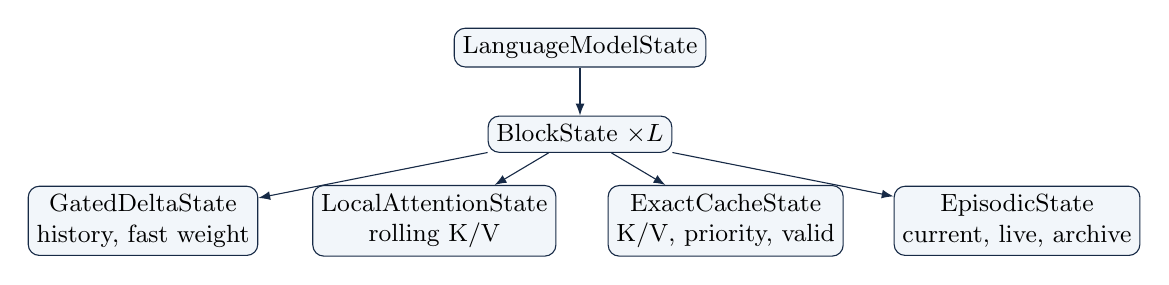
\begin{tikzpicture}[
  level distance=11mm,
  sibling distance=37mm,
  every node/.style={font=\small,draw=AlucluNavy,rounded corners,
    fill=AlucluLight,align=center,inner sep=3pt},
  edge from parent/.style={draw=AlucluNavy,-{Latex[length=1.5mm]}}
]
\node {LanguageModelState}
  child {node {BlockState \(\times L\)}
    child {node {GatedDeltaState\\history, fast weight}}
    child {node {LocalAttentionState\\rolling K/V}}
    child {node {ExactCacheState\\K/V, priority, valid}}
    child {node {EpisodicState\\current, live, archive}}};
\end{tikzpicture}
\captionof{figure}{Logical persistent-state ownership. Optional branches appear only in
scheduled layers.}
\label{fig:state-tree}
\end{center}

\subsection{Sequence, chunk, and step paths}

The same token recurrence backs three interfaces:

\begin{description}
  \item[Full sequence.] Consume a complete \(B\times T\) tensor from an
  optional incoming state and return outputs plus final state.
  \item[Chunk.] Invoke the full-sequence path repeatedly while carrying the
  returned state. This is useful for truncated backpropagation or streaming
  prefill.
  \item[Step.] Consume one token per batch item and return one-token logits and
  state.
\end{description}

In evaluation mode, the tests require these partitions to produce equivalent
outputs and terminal state within the declared numerical tolerance. Training
mode with dropout is not partition invariant because different partitions
consume random numbers in a different order.

\section{Memory Lanes and Theoretical Properties}
\label{sec:memory-lanes}
\label{sec:theory}

This section specifies the mathematical object implemented by the current
\ALUCLU reference backend.  The specification is intentionally narrower than
an abstract family of possible models: every state variable, update order, and
stabilizer below has a direct counterpart in
\texttt{src/aluclu}.  The implementation is token recurrent and uses explicit
caller-owned state.  It is therefore useful to distinguish three kinds of
statement throughout the section:
\begin{enumerate}
  \item algebraic identities of the real-arithmetic recurrence;
  \item conditional identities whose hypotheses state when numerical clamps
        are inactive; and
  \item empirical invariants exercised by the finite-precision test suite.
\end{enumerate}
In particular, ``exact'' denotes the absence of rank truncation for a retained
projected key--value record or live factor.  It does not denote unbounded,
lossless recall.

\subsection{Notation and block-level execution}
\label{subsec:notation-execution}

Let \(B\) be the batch size, \(T\) the number of tokens processed by one
call, \(d\) the model width, and \(L\) the number of residual blocks.
Table~\ref{tab:mathematical-symbols} maps the remaining symbols to the
configuration fields used by the implementation.

\begin{longtable}{@{}p{0.13\textwidth}p{0.36\textwidth}
  p{0.43\textwidth}@{}}
\caption{Symbols and their implementation counterparts.}
\label{tab:mathematical-symbols}\\
\toprule
Symbol & Code field & Meaning \\
\midrule
\endfirsthead
\toprule
Symbol & Code field & Meaning \\
\midrule
\endhead
\(H,d_k,d_v\)
  & \texttt{n\_heads}, \texttt{head\_key\_dim},
    \texttt{head\_value\_dim}
  & Number of Gated Delta heads and per-head key/value widths. \\
\(W\) & \texttt{local\_window}
  & Capacity of each local-attention rolling key--value window. \\
\(H_x,d_x,C_x\)
  & \texttt{ExactCacheConfig.n\_heads}, \(d/H_x\),
    \texttt{capacity}
  & Exact-cache head count, head width, and number of retained records. \\
\(S,K,C,A,r\)
  & \texttt{segment\_size}, \texttt{live\_segments},
    \texttt{archive\_slots}, \texttt{archive\_segments\_per\_slot},
    \texttt{archive\_rank}
  & Episodic segment length, exact-live count, archive-capsule count,
    segments per capsule, and archive rank. \\
\(d_r,p,m,J\)
  & \texttt{router\_dimension}, \texttt{router\_degree},
    \texttt{sketch\_dim}, \texttt{n\_sketches}
  & Route width, TensorSketch degree, sketch width, and number of sketches. \\
\(\kappa_g,\kappa_e\)
  & \path{GatedDeltaConfig.conv_kernel},
    \path{EpisodicMemoryConfig.conv_kernel}
  & Causal depthwise-stem kernel sizes. \\
\(f_{\min},f_{\max},\varepsilon\)
  & \texttt{feature\_floor}, \texttt{feature\_ceiling}, \texttt{eps}
  & Episodic feature bounds and numerical lower clamp. \\
\(b_x\) & \texttt{x.element\_size()}
  & Bytes per model-state scalar. \\
\bottomrule
\end{longtable}

For block \(\ell\), let \(x_{\ell,t}\in\R^d\) denote its input at token
\(t\), and define
\begin{equation}
  h_{\ell,t}=\RMSNorm(x_{\ell,t}).
  \label{eq:block-normalized-input}
\end{equation}
Every block contains a Gated Delta lane.  The local, episodic, and
residual-surprise lanes are present when, respectively,
\begin{align}
  \ell &\equiv 0
  \pmod{\texttt{local\_attention\_every}}, \\
  \ell &\equiv 0
  \pmod{\texttt{episodic\_every}}, \\
  \ell &\equiv 0
  \pmod{\texttt{exact\_cache\_every}},
\end{align}
using one-based layer indices, with the additional requirement that the
episodic or exact-cache configuration exists.  Consequently,
\begin{align}
  N_{\mathrm{local}}
    &=\left\lfloor
        \frac{L}{\texttt{local\_attention\_every}}
      \right\rfloor, \\
  N_{\mathrm{epi}}
    &=\mathbf{1}_{\{\text{episodic configured}\}}
      \left\lfloor
        \frac{L}{\texttt{episodic\_every}}
      \right\rfloor, \\
  N_{\mathrm{exact}}
    &=\mathbf{1}_{\{\text{exact cache configured}\}}
      \left\lfloor
        \frac{L}{\texttt{exact\_cache\_every}}
      \right\rfloor .
  \label{eq:scheduled-lane-counts}
\end{align}

All active lanes read the same \(h_{\ell,t}\); their outputs are not chained.
The Gated Delta lane additionally emits one scalar write-surprise value per
batch item and token.  The exact-cache lane consumes this scalar for its hard
insertion decision, but it computes its own query, key, and value projections.
Each memory lane performs its state update before reading at the same token.
Thus, the implemented convention is inclusive causal, \(j\leq t\).

\subsection{Causal depthwise streaming stems}
\label{subsec:streaming-stem}

The Gated Delta and episodic lanes each own an independent
\texttt{StreamingDepthwiseConv1d}.  For kernel width \(\kappa\), input chunk
\(x_{1:T}\), and incoming history \(c\in\R^{B\times(\kappa-1)\times d}\),
the operation is
\begin{align}
  \bar x &= [c;x_{1:T}], \\
  \widetilde x_{1:T}
    &=\operatorname{DepthwiseConv1d}_{\kappa}(\bar x), \\
  c'&=\bar x_{-(\kappa-1):}.
  \label{eq:streaming-convolution}
\end{align}
The history therefore stores exactly \(B(\kappa-1)d\) model-dtype elements.
The convolution is initialized as an identity map: all weights are zero
except the most recent causal tap, which is one, and the bias is zero.

\begin{proposition}[Chunk compositionality of the causal stem]
\label{prop:stem-compositionality}
In exact arithmetic, processing a sequence by
\eqref{eq:streaming-convolution} in any ordered partition produces the same
output sequence and terminal history as processing it in one call.
\end{proposition}
\noindent\emph{Proof sketch.}
At every boundary the state \(c'\) is exactly the suffix of length
\(\kappa-1\) required by the next causal convolution.  Each output at time
\(t\) is therefore evaluated on the same ordered \(\kappa\)-token context
under every partition.  Induction over chunk boundaries proves equality.
\hfill\(\square\)

\subsection{Gated Delta Rule-2 lane}
\label{subsec:gated-delta}

Suppress the block, batch, and head indices temporarily.  The lane applies its
own streaming stem to \(h_t\), producing \(\widetilde h_t\), and then forms
\begin{align}
  q_t
    &=\frac{W_q\widetilde h_t}
            {\max(\norm{W_q\widetilde h_t}_2,\varepsilon)}
      \in\R^{d_k}, \\
  k_t
    &=\frac{W_k\widetilde h_t}
            {\max(\norm{W_k\widetilde h_t}_2,\varepsilon)}
      \in\R^{d_k}, \\
  v_t&=W_v\widetilde h_t\in\R^{d_v}, \\
  e_t&=\sigmoid(W_e\widetilde h_t+b_e)\in(0,1)^{d_k}, \\
  w_t&=\sigmoid(W_w\widetilde h_t+b_w)\in(0,1)^{d_v}.
  \label{eq:gdr-projections}
\end{align}
Here \(e_t\) is the erase gate and \(w_t\) is the write gate.  Let
\(a=\exp(\texttt{decay\_log\_scale})>0\).  The token-dependent decay is
\begin{align}
  \log\gamma_t
    &=-a\odot
      \softplus\!\left(
        W_\gamma\widetilde h_t+\texttt{decay\_offset}
      \right), \\
  \gamma_t
    &=\max\!\left\{
        \exp(\log\gamma_t),\texttt{decay\_min}
      \right\},
  \label{eq:gdr-decay}
\end{align}
where the maximum is elementwise.  In real arithmetic,
\(\texttt{decay\_min}\leq\gamma_{t,j}<1\).

For each head, the persistent fast-weight matrix is
\(F_{t-1}\in\R^{d_k\times d_v}\).  The implemented recurrence is
\begin{align}
  \bar F_t
    &=\diag(\gamma_t)F_{t-1}, \\
  a_t&=e_t\odot k_t, \\
  \widehat v_t
    &=\bar F_t^\top a_t, \\
  v_t^{\mathrm{target}}
    &=w_t\odot v_t, \\
  \Delta v_t
    &=v_t^{\mathrm{target}}-\widehat v_t, \\
  F_t
    &=\bar F_t+k_t(\Delta v_t)^\top, \\
  o_t&=F_t^\top q_t.
  \label{eq:gdr-recurrence}
\end{align}
The outer-product update and read use the newly written \(F_t\), rather than
\(F_{t-1}\).  With head indices restored, the write-surprise scalar is
\begin{equation}
  \xi_t
  =
  \frac{
    \left(
      \sum_{h=1}^{H}\sum_{j=1}^{d_v}
      (\Delta v_{t,h,j})^2
    \right)^{1/2}
  }{\sqrt{Hd_v}}
  =
  \sqrt{
    \operatorname{mean}_{h,j}
    [(\Delta v_{t,h,j})^2]
  }.
  \label{eq:write-surprise}
\end{equation}
Thus \(\xi_t\) is an RMS write residual, not an unnormalized Euclidean norm.
The per-head output is gated and projected:
\begin{equation}
  g_t
  =
  W_{\mathrm{out}}
  \operatorname{concat}_{h=1}^{H}
  \left[
    o_{t,h}\odot
    \SiLU(W_o\widetilde h_t)_h
  \right].
  \label{eq:gdr-output}
\end{equation}
The implementation evaluates the fast-weight state, decay path, and recurrence
in fp32 even under mixed precision, then casts the stacked recurrent output
back to the model dtype before the output projection.

\begin{proposition}[Fixed recurrent state and inclusive causality]
\label{prop:gdr-state-causality}
For fixed \(H,d_k,d_v,\kappa_g,d\), the Gated Delta lane carries
\begin{equation}
  (\kappa_g-1)d
  \quad\text{model-dtype elements and}\quad
  Hd_kd_v
  \quad\text{fp32 elements}
  \label{eq:gdr-state-elements}
\end{equation}
per batch item, independently of the number of previously processed tokens.
Its output at \(t\) is a function only of inputs through \(t\), and it includes
the update induced by token \(t\).
\end{proposition}
\noindent\emph{Proof sketch.}
The only persistent tensors are the bounded convolution history and one
\(d_k\times d_v\) fast-weight matrix per head.  Every quantity on the
right-hand side of \eqref{eq:gdr-recurrence} depends on \(F_{t-1}\) and the
current stem output.  The read uses \(F_t\), establishing write-then-read
causality. \hfill\(\square\)

\subsection{Exact bounded local attention}
\label{subsec:local-attention}

Let \(H_\ell\) be the number of local-attention heads and
\(d_h=d/H_\ell\).  At token \(t\), projected \(k_t,v_t\) are appended before
the read and the cache is truncated to its last \(W\) entries:
\begin{equation}
  K_t=[K_{t-1};k_t]_{-W:},
  \qquad
  V_t=[V_{t-1};v_t]_{-W:}.
  \label{eq:local-window-update}
\end{equation}
For a retained position \(j\) and head \(h\),
\begin{equation}
  s_{t,j,h}
  =
  \frac{q_{t,h}^{\top}k_{j,h}}{\sqrt{d_h}}
  -
  \softplus(\texttt{slope\_raw}_h)(t-j),
  \label{eq:local-score}
\end{equation}
where the implementation constructs \(t-j\) as the reverse distance within
the rolling window.  It then computes
\begin{align}
  \alpha_{t,:,h}
    &=\softmax(s_{t,:,h}), \\
  \ell_{t,h}
    &=\sum_{j\in\mathcal W_t}\alpha_{t,j,h}v_{j,h},
  \qquad
  \mathcal W_t=\{\max(1,t-W+1),\ldots,t\}.
  \label{eq:local-read}
\end{align}
The softmax is explicitly evaluated in fp32 and cast back to the model dtype.
Attention-weight dropout is applied only in training mode.

\begin{proposition}[Local exactness and bound]
\label{prop:local-exactness}
The local lane computes ordinary causal softmax attention, with the learned
linear recency bias in \eqref{eq:local-score}, over exactly the retained
window \(\mathcal W_t\).  At saturation its persistent key--value payload is
\begin{equation}
  F_{\mathrm{local}}=2dW
  \label{eq:local-state-elements}
\end{equation}
model-dtype elements per batch item, and its attention read costs
\(\bigO(dW)\) per token, excluding dense projections.
\end{proposition}
\noindent\emph{Proof sketch.}
Equation~\eqref{eq:local-window-update} retains no index earlier than
\(t-W+1\), and it inserts the current key and value before
\eqref{eq:local-read}.  The softmax is not kernelized or low-rank
approximated.  Two tensors of shape \(H_\ell\times W\times d_h\) yield
\(2dW\) elements. \hfill\(\square\)

\subsection{Residual-surprise exact key--value cache}
\label{subsec:exact-cache}

The exact cache has independent projections
\begin{equation}
  q_t^x=W_q^x h_t,\qquad
  k_t^x=W_k^x h_t,\qquad
  v_t^x=W_v^x h_t,
  \label{eq:exact-cache-projections}
\end{equation}
split into \(H_x\) heads of width \(d_x=d/H_x\).  It receives the scalar
\(\xi_t\) from \eqref{eq:write-surprise}; no separate learned priority
projection is present.

\subsubsection{Hard insertion rule}

For each batch item, the state contains \(C_x\) key slots, value slots,
priorities, and valid bits.  Let
\begin{equation}
  \mathcal E_t
  =
  \{j:\neg\texttt{valid}_{t-1,j}\}.
\end{equation}
If \(\mathcal E_t\neq\varnothing\), the implementation selects the first
invalid slot.  Otherwise it selects
\begin{equation}
  j_{\min}
  =
  \arg\min_{1\leq j\leq C_x}
  \texttt{priority}_{t-1,j}.
\end{equation}
The comparison priority is detached from autograd and converted to the
priority dtype:
\begin{equation}
  \widehat\xi_t=\stopgrad(\xi_t).
\end{equation}
The write predicate is
\begin{equation}
  \operatorname{write}_t
  =
  \mathbf{1}\{\mathcal E_t\neq\varnothing\}
  \lor
  \mathbf{1}\{
    \widehat\xi_t>
    \texttt{priority}_{t-1,j_{\min}}
  \}.
  \label{eq:exact-cache-write}
\end{equation}
The inequality is strict: an equal-priority arrival does not replace the
older retained record.  All heads write the current projected key and value to
the same selected slot.

\begin{proposition}[Stable top-\(C_x\) priority invariant]
\label{prop:top-cx}
Assume finite priorities and process one batch item in temporal order.  After
\(t\) updates, the cache contains \(\min(C_x,t)\) records whose priorities are
the largest priorities seen so far, with earlier records retained at the
cutoff when priorities tie.
\end{proposition}
\noindent\emph{Proof sketch.}
Before saturation every arrival occupies one empty position.  After
saturation, an arrival below or equal to the current minimum cannot belong to
a strictly better top-\(C_x\) set and is rejected.  An arrival above the
minimum replaces exactly one minimum.  Induction on \(t\) gives the invariant;
strict comparison yields stable earlier-tie retention. \hfill\(\square\)

\subsubsection{Write-then-read exact softmax}

Insertion precedes the current read.  For valid slot \(j\),
\begin{align}
  s_{t,h,j}^x
    &=
    \frac{(q_{t,h}^x)^\top k_{j,h}^x}{\sqrt{d_x}}, \\
  \alpha_{t,h,:}^x
    &=\softmax(s_{t,h,:}^x), \\
  o_{t,h}^x
    &=\sum_{j:\mathrm{valid}_j}
      \alpha_{t,h,j}^x v_{j,h}^x.
  \label{eq:exact-cache-read}
\end{align}
Invalid positions are masked with the minimum finite value of the score dtype.
The first token is always inserted because capacity is positive and an empty
slot exists, so every read has at least one valid entry.  Half and bfloat16
scores use fp32 softmax; float32 and float64 scores retain their score dtype.
The current record participates in its read if accepted.  If rejected, its
query still reads the retained past, but its key and value are absent.

The selection path is deliberately non-differentiable:
\(\widehat\xi_t\) is detached, and integer indexing plus one-hot selection
implements the replacement.  Accepted key/value projections receive gradient
through \eqref{eq:exact-cache-read}; the cache loss does not backpropagate
through the discrete ranking decision into \(\xi_t\).

\begin{remark}[Meaning of exactness]
The cache stores the projected \(k_t^x,v_t^x\) of accepted records without
rank truncation or averaging.  It does not store all tokens, raw hidden states,
token identifiers, or any record rejected or later evicted by
\eqref{eq:exact-cache-write}.
\end{remark}

Its logical state size per batch item is
\begin{equation}
  F_{\mathrm{exact}}
  =
  2C_xd+2C_x.
  \label{eq:exact-cache-state-elements}
\end{equation}
For ordinary fp16, bfloat16, or fp32 model state, priority is fp32 and valid is
Boolean, so the byte payload is
\begin{equation}
  \operatorname{bytes}_{\mathrm{exact},B=1}
  =
  2b_xC_xd+5C_x.
  \label{eq:exact-cache-state-bytes}
\end{equation}
In the float64 validation path priority is also float64, replacing \(5C_x\)
by \(9C_x\).  Full-shape \texttt{torch.where} updates and the softmax read
both cost \(\bigO(C_xd)\) per token, excluding dense projections.

\subsection{Bounded episodic associative memory}
\label{subsec:episodic-memory}

The episodic lane applies its own causal stem to \(h_t\), yielding
\(\widetilde h_t^e\), and uses a bounded positive feature map
\begin{equation}
  \phi(a)
  =
  f_{\min}+(f_{\max}-f_{\min})\sigmoid(a),
  \qquad
  0<f_{\min}<f_{\max}.
  \label{eq:positive-feature-map}
\end{equation}
The implementation computes
\begin{align}
  q_t^+&=\phi(W_q^e\widetilde h_t^e), \\
  k_t^+&=\phi(W_k^e\widetilde h_t^e), \\
  v_t^e&=W_v^e\widetilde h_t^e.
  \label{eq:episodic-projections}
\end{align}
Componentwise,
\begin{equation}
  f_{\min}\leq \phi(a)_j\leq f_{\max},
  \label{eq:feature-bounds}
\end{equation}
where equality can occur through floating-point sigmoid saturation.

\subsubsection{Separate numerator and denominator summaries}

For a retained token set \(\mathcal I_i\), slot \(i\) represents
\begin{align}
  M_i
    &=\sum_{t\in\mathcal I_i}
      v_t^e(k_t^+)^\top, \\
  z_i
    &=\sum_{t\in\mathcal I_i}k_t^+.
  \label{eq:slot-moments}
\end{align}
The numerator is stored in factors
\begin{equation}
  M_i
  =
  L_i^\top R_i,
  \qquad
  L_i,R_i\in\R^{f_i\times d},
  \label{eq:slot-factorization}
\end{equation}
corresponding to the code fields \texttt{left} and \texttt{right}.  For an
exact current or live segment, one factor row corresponds to one token.  The
slot read is
\begin{align}
  n_i(q_t^+)
    &=M_iq_t^+
      =L_i^\top(R_iq_t^+), \\
  d_i(q_t^+)
    &=z_i^\top q_t^+.
  \label{eq:slot-read}
\end{align}
The denominator is never reconstructed from \(R_i\).  After SVD truncation,
\(R_i\) is a signed low-rank factor and is not a collection of positive keys.
The independent \(z_i\) is therefore the sole valid denominator summary.

\begin{proposition}[Positive denominator and compression separation]
\label{prop:positive-denominator}
Every nonempty retained slot satisfies
\begin{equation}
  d_i(q_t^+)>0
\end{equation}
in real arithmetic.  Rank truncation of \(M_i\) changes only the numerator in
\eqref{eq:slot-read}; it does not change \(z_i\) or \(d_i\).
\end{proposition}
\noindent\emph{Proof sketch.}
Every component of every retained \(k_t^+\) and of \(q_t^+\) is positive by
\eqref{eq:positive-feature-map}.  Hence \(z_i\) is componentwise positive and
its inner product with \(q_t^+\) is positive.  The compression routines replace
only \texttt{left} and \texttt{right}; they copy or add \(z_i\) directly.
\hfill\(\square\)

\subsubsection{Route features and TensorSketch}

The route vector is
\begin{equation}
  u_t
  =
  \frac{W_r\widetilde h_t^e}
       {\max(\norm{W_r\widetilde h_t^e}_2,\varepsilon)}
  \in\R^{d_r}.
  \label{eq:route-vector}
\end{equation}
Thus \(\norm{u_t}_2=1\) when the pre-normalization norm is at least
\(\varepsilon\), and \(\norm{u_t}_2\leq 1\) otherwise.

For sketch \(j\in\{1,\ldots,J\}\), degree factor
\(a\in\{1,\ldots,p\}\), bucket \(b\in\{0,\ldots,m-1\}\), fixed hash
\(h_{j,a}\), and fixed sign map \(s_{j,a}\), define
\begin{equation}
  \operatorname{CS}_{j,a}(u)[b]
  =
  \sum_{\ell:h_{j,a}(\ell)=b}
  s_{j,a}(\ell)u_\ell .
  \label{eq:count-sketch}
\end{equation}
The implemented TensorSketch feature is
\begin{equation}
  \psi_j(u)
  =
  \operatorname{IFFT}\!\left(
    \prod_{a=1}^{p}
    \operatorname{FFT}(
      \operatorname{CS}_{j,a}(u)
    )
  \right)
  \in\R^m.
  \label{eq:tensor-sketch}
\end{equation}
Hashes and signs are generated once from \texttt{router\_seed} and registered
as persistent buffers.  A slot stores additive summaries
\begin{align}
  r_i&=\sum_{t\in\mathcal I_i}u_t, \\
  \Psi_{i,j}
    &=\sum_{t\in\mathcal I_i}\psi_j(u_t), \\
  c_i&=\abs{\mathcal I_i}.
  \label{eq:route-summaries}
\end{align}
The sketch is used only to score slots.  Finite \(m\) and \(J\) permit
collisions, and the implementation does not claim a collision-free identity
store.  Configuration validation requires odd \(J\), making the median below
unambiguous.

\subsubsection{Mass-weighted routing and its clamp condition}

For route query \(u_q\) and slot \(i\), the linear and polynomial scores are
\begin{align}
  \ell_i
    &=
    \frac{u_q^\top r_i}{\sqrt{\max(c_i,1)}}, \\
  \rho_i
    &=
    \frac{
      \median_{j=1,\ldots,J}
      [\psi_j(u_q)^\top\Psi_{i,j}]
    }{\sqrt{\max(c_i,1)}}.
  \label{eq:route-component-scores}
\end{align}
Let
\begin{equation}
  (\pi_1,\pi_p)=\softmax(\texttt{mix\_logits}),
  \qquad
  s_i=\pi_1\ell_i+\pi_p\rho_i.
  \label{eq:mixed-route-score}
\end{equation}
The signed, bounded temperature is
\begin{equation}
  \theta
  =
  \texttt{max\_temperature}
  \tanh(\texttt{temperature\_raw}).
  \label{eq:router-temperature}
\end{equation}
The implementation does not constrain \(\theta\) to be positive.

It is important to state the numerical stabilizers exactly.  With
\begin{align}
  D_0&=\sum_i d_i, \\
  D_\varepsilon&=\max(D_0,\varepsilon), \\
  \bar s
    &=\frac{\sum_i s_i d_i}{D_\varepsilon}, \\
  \eta_i
    &=\clip\!\left(
       \theta(s_i-\bar s),-L_w,L_w
      \right), \\
  \widetilde w_i&=\exp(\eta_i)>0, \\
  c_\varepsilon
    &=\max\!\left(
      \frac{\sum_i\widetilde w_i d_i}{D_\varepsilon},
      \varepsilon
    \right), \\
  w_i&=\frac{\widetilde w_i}{c_\varepsilon},
  \qquad
  L_w=\texttt{max\_log\_weight},
  \label{eq:implemented-router}
\end{align}
the routed numerator and returned denominator are
\begin{align}
  N_{\mathrm{route}}
    &=\sum_iw_i n_i, \\
  D_{\mathrm{returned}}
    &=D_0, \\
  y_t^e
    &=\frac{N_{\mathrm{route}}}
            {\max(D_{\mathrm{returned}},\varepsilon)}.
  \label{eq:episodic-output}
\end{align}
The code intentionally does not multiply the returned denominator by \(w_i\).

\begin{proposition}[Conditional denominator-mass conservation]
\label{prop:conditional-mass}
If both lower clamps in \eqref{eq:implemented-router} are inactive, namely
\begin{equation}
  D_0\geq\varepsilon
  \quad\text{and}\quad
  \frac{\sum_i\widetilde w_i d_i}{D_0}
  \geq\varepsilon,
  \label{eq:mass-conservation-conditions}
\end{equation}
then
\begin{equation}
  w_i>0,
  \qquad
  \sum_iw_id_i=D_0.
  \label{eq:mass-conservation}
\end{equation}
If additionally \(\theta=0\), then \(w_i=1\) for every slot.
\end{proposition}
\noindent\emph{Proof sketch.}
Under \eqref{eq:mass-conservation-conditions},
\[
  c_\varepsilon
  =
  \frac{\sum_i\widetilde w_i d_i}{D_0}.
\]
Substitution into \(w_i=\widetilde w_i/c_\varepsilon\) yields
\(\sum_iw_id_i=D_0\); positivity follows from the exponential and positive
normalizer.  When \(\theta=0\), every \(\eta_i=0\), hence
\(\widetilde w_i=1\) and \(c_\varepsilon=1\). \hfill\(\square\)

\begin{remark}[Active-clamp behavior]
\label{rem:active-clamp}
When either condition in \eqref{eq:mass-conservation-conditions} fails, the
implemented stabilized formula remains \eqref{eq:implemented-router}, but
\eqref{eq:mass-conservation} is not an unconditional identity.  For example,
if only the first clamp is active and the second is inactive, then
\(\sum_iw_id_i=D_\varepsilon\), not necessarily \(D_0\).  This distinction is
why all exact mass-conservation claims in this paper carry the inactive-clamp
hypothesis.  The unit test exercises positive masses well above
\(\varepsilon\) and verifies the equality to floating-point tolerance.
\end{remark}

\subsubsection{Current, live, and archive lifecycle}

Each token first creates a one-row slot and is appended to
\texttt{current}.  When the current factor count reaches \(S\), the completed
slot moves to the end of the exact \texttt{live} tuple and
\texttt{current} becomes empty.  If this produces more than \(K\) live
segments, the oldest live segment is evicted.  When \(C=0\), that segment is
forgotten.  Otherwise it enters a temporal archive ring:
\begin{enumerate}
  \item the first segment of a capsule is compressed to rank \(r\);
  \item further incoming segments are merged into the active capsule until it
        contains \(A\) segments;
  \item the cursor then advances to the next capsule; and
  \item once all \(C\) positions exist, advancing overwrites the next capsule
        and erases its former contents.
\end{enumerate}
The physical tuple order is not required to be chronological; the cursor
identifies the active ring position.

The method \texttt{maximum\_retained\_tokens()} returns the conservative
allocation-style horizon
\begin{equation}
  H_{\max}
  =
  S(1+K+CA)
  =
  \underbrace{S}_{\text{current budget}}
  +
  \underbrace{KS}_{\text{exact live}}
  +
  \underbrace{CAS}_{\text{compressed archive}}.
  \label{eq:retained-horizon}
\end{equation}
Because a current segment is sealed immediately at \(S\),
\begin{equation}
  0\leq\abs{\texttt{current}}<S,
  \qquad
  N_{\mathrm{retained}}\leq H_{\max}-1
  \label{eq:reachable-retained-horizon}
\end{equation}
for an actually reachable state.  After a full-ring overwrite, the number of
archived segments falls from \(CA\) to \((C-1)A+1\), then rises as the new
active capsule fills.  Hence the age horizon has a sawtooth variation of up to
\(A-1\) archived segments.

\begin{proposition}[Bounded episodic lifecycle]
\label{prop:bounded-episodic-lifecycle}
For every stream length,
\begin{equation}
  \abs{\texttt{live}}\leq K,\qquad
  \abs{\texttt{archive}}\leq C,\qquad
  \texttt{archive\_cursor\_segments}\leq A,
  \label{eq:episodic-container-bounds}
\end{equation}
and \eqref{eq:reachable-retained-horizon} holds.  Current and live numerator
factors are algebraically exact sums for their retained tokens; archive
numerators have rank at most \(r\); overwritten capsules have no remaining
representation.
\end{proposition}
\noindent\emph{Proof sketch.}
Sealing resets current before it can exceed \(S-1\).  Live overflow immediately
evicts its oldest element, maintaining \(K\).  Archive insertion either merges
into the current capsule, appends while fewer than \(C\) capsules exist, or
overwrites one existing capsule.  The cursor advances after \(A\) segments.
These transitions establish \eqref{eq:episodic-container-bounds} by induction;
counting their maximum represented tokens yields
\eqref{eq:reachable-retained-horizon}. \hfill\(\square\)

\subsection{Thin-QR, small-core SVD compression}
\label{subsec:small-core-svd}

The archive compresses a factor pair without materializing a dense
\(d\times d\) numerator.  Suppress the batch index and let
\begin{equation}
  L=\texttt{left}^{\top}\in\R^{d\times F},
  \qquad
  R=\texttt{right}^{\top}\in\R^{d\times F},
  \qquad
  M=LR^\top.
  \label{eq:compression-input}
\end{equation}
Reduced QR decompositions give
\begin{equation}
  L=Q_LR_L,\qquad
  R=Q_RR_R.
\end{equation}
The code performs an SVD only on
\begin{equation}
  C_{\mathrm{core}}
  =
  R_LR_R^\top
  =
  U_c\Sigma V_c^\top.
  \label{eq:small-core}
\end{equation}
If \(p_c=\min(d,F)\), then \(C_{\mathrm{core}}\in\R^{p_c\times p_c}\).
Let
\begin{equation}
  r_{\mathrm{eff}}
  =
  \min(r,\operatorname{len}(\Sigma)).
\end{equation}
The returned factors are
\begin{align}
  \widehat L_{\mathrm{rows}}
    &=
    \left(
      Q_LU_{c,:r_{\mathrm{eff}}}
      \Sigma_{:r_{\mathrm{eff}}}^{1/2}
    \right)^\top, \\
  \widehat R_{\mathrm{rows}}
    &=
    \left(
      Q_RV_{c,:r_{\mathrm{eff}}}
      \Sigma_{:r_{\mathrm{eff}}}^{1/2}
    \right)^\top.
  \label{eq:compressed-factors}
\end{align}
Zero rows pad each factor to exactly \(r\), keeping archive shapes static.
For half or bfloat16 input the QR and SVD work in fp32 before results are cast
back; float32 and float64 retain their input work dtype.

\begin{proposition}[Best rank-\(r\) numerator in exact arithmetic]
\label{prop:best-rank}
Ignoring finite-precision QR/SVD and the final dtype cast, the reconstructed
\begin{equation}
  \widehat M
  =
  \widehat L_{\mathrm{rows}}^\top
  \widehat R_{\mathrm{rows}}
\end{equation}
is a best rank-\(r_{\mathrm{eff}}\) approximation to \(M\) in Frobenius norm,
and
\begin{equation}
  \norm{M-\widehat M}_F
  =
  \delta
  =
  \left(
    \sum_{j>r_{\mathrm{eff}}}\sigma_j(C_{\mathrm{core}})^2
  \right)^{1/2}.
  \label{eq:discarded-tail}
\end{equation}
If \(r\geq\rank(M)\), the compression is algebraically exact.
\end{proposition}
\noindent\emph{Proof sketch.}
Reduced QR factors have orthonormal columns, so left and right multiplication
by \(Q_L,Q_R^\top\) preserves all nonzero singular values and Frobenius norms.
Truncating the SVD of \(C_{\mathrm{core}}\) therefore gives the
Eckart--Young best-rank approximation to \(M\).  Splitting
\(\Sigma^{1/2}\) symmetrically reconstructs that truncation.
\hfill\(\square\)

In a typical merge, an existing rank-\(r\) capsule is concatenated with an
exact \(S\)-row live segment, so \(F\leq r+S\) and
\begin{equation}
  p_c=\min(d,F)\leq\min(d,r+S).
\end{equation}
One merge costs approximately
\begin{equation}
  \bigO(dFp_c+p_c^3).
  \label{eq:compression-merge-cost}
\end{equation}
Since a live overflow occurs at most once every \(S\) tokens, its steady-state
amortized cost is
\begin{equation}
  \bigO\!\left(
    \frac{d(r+S)p_c+p_c^3}{S}
  \right)
  \quad\text{per token}.
  \label{eq:compression-amortized-cost}
\end{equation}
The core is genuinely small only when \(r+S\ll d\).  Configuration validation
enforces \(r\leq d\), but does not enforce \(r+S<d\); the core can therefore
grow to \(d\times d\).

\subsection{Compression error ledger}
\label{subsec:error-ledger}

For one archive capsule, let \(M_1,\ldots,M_u\) be exact incoming segment
numerators and
\begin{equation}
  M_u^\star=\sum_{j=1}^{u}M_j
\end{equation}
the ideal retained numerator.  At merge \(u\), the implementation truncates
\begin{equation}
  A_u=\widehat M_{u-1}+M_u,
  \qquad
  \widehat M_u=P_r(A_u),
\end{equation}
and reports
\begin{equation}
  \delta_u
  =
  \norm{A_u-P_r(A_u)}_F
  =
  \left(
    \sum_{j>r}\sigma_j(A_u)^2
  \right)^{1/2}.
  \label{eq:merge-tail}
\end{equation}
The slot field \texttt{error\_bound} is updated linearly:
\begin{equation}
  E_u
  =
  E_{u-1}+E_{\mathrm{incoming}}+\delta_u.
  \label{eq:error-ledger-update}
\end{equation}
For a freshly evicted exact live segment,
\(E_{\mathrm{incoming}}=0\).

\begin{proposition}[Retained-capsule error bound]
\label{prop:error-ledger}
In exact arithmetic, the ledger satisfies
\begin{equation}
  \norm{M_u^\star-\widehat M_u}_F\leq E_u.
  \label{eq:ledger-frobenius-bound}
\end{equation}
Consequently, for any query \(q\),
\begin{equation}
  \norm{(M_u^\star-\widehat M_u)q}_2
  \leq E_u\norm{q}_2.
  \label{eq:ledger-query-bound}
\end{equation}
\end{proposition}
\noindent\emph{Proof sketch.}
Write
\[
  M_u^\star-\widehat M_u
  =
  (M_{u-1}^\star-\widehat M_{u-1})
  +(M_u-\widehat M_{\mathrm{incoming}})
  +(A_u-P_r(A_u)).
\]
The triangle inequality and the inductive bounds on the first two terms yield
\eqref{eq:ledger-frobenius-bound} with the additive update
\eqref{eq:error-ledger-update}.  Submultiplicativity,
\(\norm{Eq}_2\leq\norm{E}_F\norm{q}_2\), yields
\eqref{eq:ledger-query-bound}. \hfill\(\square\)

Because \(z_i\), route sums, sketch sums, and counts are accumulated separately
from numerator compression, the ideal and compressed reads use the same
denominator and router weights when compared at the same retained segmentation.
For positive \(w_i\),
\begin{equation}
  \norm{y^\star-\widehat y}_2
  \leq
  \frac{
    \norm{q}_2
    \sum_{i\in\mathrm{archive}}w_iE_i
  }{D_0},
  \label{eq:routed-output-error-bound}
\end{equation}
provided the mathematical denominator is \(D_0>0\).  This bound covers only
currently retained capsules.  It excludes overwritten history, finite-precision
QR/SVD error, rounding from casting factors back to a lower dtype, and any task
accuracy or recall guarantee.

\subsection{Token-wise branch fusion and SwiGLU}
\label{subsec:fusion}

Let \(b_{t,j}\in\R^d\) denote active branch \(j\)'s output.  Each branch has an
independent RMS normalization and an unconstrained learned scalar:
\begin{equation}
  \widetilde b_{t,j}
  =
  \beta_j\RMSNorm_j(b_{t,j}),
  \qquad
  \beta_j=\texttt{branch\_scale}_j.
  \label{eq:branch-normalization}
\end{equation}
When more than one branch is active,
\begin{align}
  \alpha_t
    &=\softmax(W_fh_t+b_f), \\
  f_t
    &=\sum_j\alpha_{t,j}\widetilde b_{t,j},
  \qquad
  \alpha_{t,j}>0,\quad
  \sum_j\alpha_{t,j}=1.
  \label{eq:convex-fusion}
\end{align}
With a single branch, the fusion projection is absent and the normalized,
scaled branch is returned directly.  For a multi-branch block, \(W_f,b_f\)
are initialized to zero and every \(\beta_j\) to one, giving a uniform mixture
at initialization.

\begin{proposition}[Precise convexity statement]
\label{prop:fusion-convexity}
For each token, \(f_t\) lies in the convex hull of the scaled normalized
vectors \(\{\widetilde b_{t,j}\}_j\).  It is not generally constrained to the
convex hull of the raw branch outputs \(\{b_{t,j}\}_j\).
\end{proposition}
\noindent\emph{Proof sketch.}
Softmax gives positive coefficients summing to one, proving the first claim.
The second follows because each \(\beta_j\) is unconstrained and each branch
has a distinct nonlinear RMS normalization. \hfill\(\square\)

The first residual update is
\begin{equation}
  x'_t
  =
  x_t+\operatorname{Dropout}(f_t).
\end{equation}
Writing
\begin{equation}
  (g_t^{\mathrm{ffn}},v_t^{\mathrm{ffn}})
  =
  \operatorname{split}\!\left(
    W_{\mathrm{in}}\RMSNorm(x'_t)
  \right),
\end{equation}
the feed-forward output and second residual are
\begin{align}
  \operatorname{SwiGLU}(x'_t)
    &=
    W_{\mathrm{out}}^{\mathrm{ffn}}
    \left[
      \SiLU(g_t^{\mathrm{ffn}})
      \odot v_t^{\mathrm{ffn}}
    \right], \\
  x_{t,\mathrm{out}}
    &=
    x'_t+
    \operatorname{Dropout}(
      \operatorname{SwiGLU}(x'_t)
    ).
  \label{eq:block-output}
\end{align}

\subsection{Global causality and chunk/step equivalence}
\label{subsec:causality-chunking}

Let a lane state transition be written
\[
  (y_t,\state_t)=\mathcal T(x_t,\state_{t-1}).
\]
The concrete \(\state_t\) is the tuple of convolution histories, Gated Delta
fast weights, local key--value windows, exact-cache tensors and metadata, and
episodic current/live/archive state.

\begin{proposition}[Inclusive causal block semantics]
\label{prop:global-causality}
With fixed parameters and incoming state, the output at token \(t\) depends
only on the incoming state and tokens through \(t\).  No future token can
change an earlier output.  The current token can influence its own memory
read in every memory lane.
\end{proposition}
\noindent\emph{Proof sketch.}
The streaming stems are causal by
\eqref{eq:streaming-convolution}.  The Gated Delta lane updates \(F_t\) before
reading it; local attention appends \((k_t,v_t)\) before softmax; the exact
cache decides insertion before reading; and the episodic lane writes and
performs any seal, eviction, merge, or overwrite before aggregating its slots.
Fusion and SwiGLU are token local.  Composition over layers preserves
causality. \hfill\(\square\)

The language-model loss uses
\(\texttt{logits[:, :-1]}\) against \(\texttt{labels[:, 1:]}\), so the
inclusive memory read is compatible with next-token prediction.

\begin{proposition}[Chunk and step equivalence]
\label{prop:chunk-step}
Assume evaluation mode, fixed parameters, identical initial state, exact
arithmetic, and the same token order.  For any ordered partition of a sequence,
concatenating chunk outputs yields the same outputs and terminal state as one
full call or repeated one-token \texttt{step} calls.
\end{proposition}
\noindent\emph{Proof sketch.}
Each forward method applies the same token transition in temporal order.
Proposition~\ref{prop:stem-compositionality} handles both convolutional stems.
All other state updates are functions solely of the previous explicit state
and current projected token.  Associating the composition
\(\mathcal T_T\circ\cdots\circ\mathcal T_1\) according to chunk boundaries
does not change it. \hfill\(\square\)

\begin{remark}[Finite precision and training mode]
The implementation tests chunk/step equality in evaluation mode with numerical
tolerances, because vectorized linear projections and convolution kernels may
have shape-dependent floating-point reduction order.  In training mode,
different partitioning can also consume dropout random numbers differently.
Therefore Proposition~\ref{prop:chunk-step} is not stated as bitwise equality
for arbitrary training executions.
\end{remark}

\subsection{Persistent-state and compute bounds}
\label{subsec:state-compute}

Define the full conservative current/live slot size
\begin{equation}
  F_{\mathrm{live}}
  =
  2Sd+d+d_r+Jm+2,
  \label{eq:live-slot-size}
\end{equation}
and archive slot size
\begin{equation}
  F_{\mathrm{archive}}
  =
  2rd+d+d_r+Jm+2.
  \label{eq:archive-slot-size}
\end{equation}
The terms are the two numerator factors, exact \(z\), route sum, \(J\) sketch
sums, count, and error ledger.  The episodic state bound per batch item is
\begin{equation}
  F_{\mathrm{epi}}
  =
  (K+1)F_{\mathrm{live}}
  +CF_{\mathrm{archive}}
  +(\kappa_e-1)d.
  \label{eq:episodic-state-bound}
\end{equation}
This is conservative because a reachable current slot has fewer than \(S\)
rows.  The temporary fp32 QR/SVD workspace is not persistent state.

Combining all scheduled lanes gives the following logical tensor-byte bound
per batch item for ordinary non-float64 execution:
\begin{align}
  \operatorname{bytes}_{B=1}
  \leq{}&
  L\left[
    b_x(\kappa_g-1)d
    +4Hd_kd_v
  \right]
  +
  N_{\mathrm{local}}(2b_xdW)
  \nonumber\\
  &+
  N_{\mathrm{epi}}(b_xF_{\mathrm{epi}})
  +
  N_{\mathrm{exact}}
  \left(
    2b_xC_xd+5C_x
  \right).
  \label{eq:model-state-byte-bound}
\end{align}
Batch size \(B\) multiplies the tensor payload by \(B\).  This accounting
excludes parameters, optimizer state, autograd activations, QR/SVD workspace,
Python metadata, allocator fragmentation, and excess backing-storage
capacity.  In particular, bounded inference state does not imply bounded
training activation memory when the entire computation graph is retained.

Table~\ref{tab:lane-complexity} summarizes token costs.  Dense projection costs
are shown separately because the persistent-memory terms are the quantities
that distinguish the four lanes.

\begin{table}[t]
\centering
\small
\caption{Per-token time and persistent state for fixed configuration.}
\label{tab:lane-complexity}
\begin{tabularx}{\linewidth}{@{}l X X@{}}
\toprule
Lane & Per-token time beyond or including stated projections
     & Persistent elements per batch item \\
\midrule
Gated Delta
  & \(\bigO(Hd_kd_v+\kappa_gd)\) recurrence/stem, plus its dense
    query/key/value/gate projections
  & \(Hd_kd_v\) fp32 plus \((\kappa_g-1)d\) model-dtype \\
Local exact
  & \(\bigO(dW)\) attention plus \(\bigO(d^2)\) QKV/output projections
  & \(2dW\) model-dtype \\
Residual-surprise exact
  & \(\bigO(C_xd)\) selection, full-shape update, and read, plus
    \(\bigO(d^2)\) projections
  & \(2C_xd\) model-dtype plus \(C_x\) priority and \(C_x\) valid entries \\
Episodic
  & Factor read, routing, sketching, dense projections, and amortized
    compression as in \eqref{eq:episodic-token-cost}
  & At most \(F_{\mathrm{epi}}\) model-dtype elements \\
\bottomrule
\end{tabularx}
\end{table}

At most \(1+K+C\) episodic slots participate in a read.  Their factor-read
cost is
\begin{equation}
  \bigO\!\left(
    d[S(K+1)+Cr]
  \right).
\end{equation}
Route comparisons cost
\begin{equation}
  \bigO\!\left(
    (K+C+1)(d_r+Jm)
  \right),
\end{equation}
and the current FFT implementation constructs a token sketch in
\begin{equation}
  \bigO\!\left(
    Jp[d_r+m\log m]
  \right).
\end{equation}
Including amortized compression but suppressing dense projection constants,
\begin{equation}
  \begin{split}
  \operatorname{cost}_{\mathrm{epi/token}}
  =\bigO\bigg(
    &d[S(K+1)+Cr]
    +(K+C+1)(d_r+Jm)\\
    &+Jp[d_r+m\log m]
    +\frac{d(r+S)p_c+p_c^3}{S}
  \bigg).
  \end{split}
  \label{eq:episodic-token-cost}
\end{equation}
For a fixed configuration, recurrent-decode cost and persistent state are
independent of total context length.  A \(T\)-token scan nevertheless costs
\(\bigO(T)\) times the fixed per-token work.  The current Python backend uses
token loops, tuple concatenation, full-cache \texttt{torch.where}, and
occasional QR/SVD; these asymptotic state bounds do not imply fused-kernel
throughput.

\subsection{Finite-capacity boundary}
\label{subsec:finite-capacity}

Every persistent lane is explicitly bounded:
\begin{itemize}
  \item Gated Delta has \(Hd_kd_v\) fp32 fast-weight elements;
  \item local attention stores only the last \(W\) projected key--value pairs;
  \item the residual-surprise cache stores at most \(C_x\) selected projected
        key--value pairs; and
  \item episodic memory stores one partial segment, at most \(K\) exact live
        segments, and at most \(C\) rank-\(r\) archive capsules.
\end{itemize}
For every capsule,
\begin{equation}
  \rank(\widehat M_i)\leq r.
\end{equation}
Exact \(z_i\), route, sketch, and count summaries cannot reconstruct numerator
directions discarded by rank truncation.

\begin{proposition}[Finite-state impossibility of arbitrary unbounded recall]
\label{prop:finite-state-impossibility}
Fix model parameters and a persistent state representation with at most
\(Q\) physical bits.  Suppose query keys are supplied externally and each of
\(N\) independent associated values belongs to an alphabet
\(\mathcal V\), with \(\abs{\mathcal V}\geq2\).  A system that recalls every
possible assignment without error must satisfy
\begin{equation}
  Q\geq N\log_2\abs{\mathcal V},
  \qquad\text{equivalently}\qquad
  N\leq\frac{Q}{\log_2\abs{\mathcal V}}.
  \label{eq:finite-state-bound}
\end{equation}
\end{proposition}
\noindent\emph{Proof sketch.}
There are \(\abs{\mathcal V}^N\) possible independent value assignments.
Perfect recall requires that assignments needing different answers not collapse
to the same persistent state.  A \(Q\)-bit state has at most \(2^Q\) distinct
physical encodings, so injectivity requires
\(2^Q\geq\abs{\mathcal V}^N\).  Taking base-two logarithms yields
\eqref{eq:finite-state-bound}. \hfill\(\square\)

This counting bound is deliberately optimistic: it ignores floating-point
noise, hash collisions, readout interference, rank limits, replacement, and
optimization error.  The implemented consequences are concrete.  Exact-cache
records outside the stable top-\(C_x\) set are absent from that lane;
local-attention records older than \(W\) are absent from that lane; an
overwritten episodic capsule is absent entirely; and retained archive
numerators are generally lossy.  Increasing \(A\) extends
\eqref{eq:retained-horizon} without adding archive slots, but forces more
segments through the same rank-\(r\) capsule and can only increase the
opportunity for approximation and interference.  No equation in this section
supports exact recall over an unbounded stream.

\subsection{Code correspondence and validation boundary}
\label{subsec:code-correspondence}

The equations above were cross-checked against the following implementation
sites:
\begin{itemize}
  \item \texttt{gated\_delta.py}: decay, erase/write recurrence, RMS surprise,
        fp32 fast weights, and write-then-read order;
  \item \texttt{local\_attention.py}: append/truncate/read order, learned
        recency slope, fp32 softmax, and \(W\)-bounded state;
  \item \texttt{exact\_cache.py}: detached strict replacement, batch-local
        first-empty/minimum selection, exact softmax read, and mixed-dtype
        state accounting;
  \item \texttt{episodic.py}: positive feature map, separate \(M\) and \(z\),
        TensorSketch routing, stabilized mass normalization, ring lifecycle,
        retained horizon, and state formula;
  \item \texttt{compression.py}: reduced QR, small-core SVD, symmetric singular
        split, discarded tail, and additive error ledger;
  \item \texttt{model.py}: parallel branch execution, token-wise softmax
        fusion, residual ordering, and SwiGLU; and
  \item \texttt{state.py}: the exact persistent tensor fields counted in
        \eqref{eq:model-state-byte-bound}.
\end{itemize}

The corresponding tests check Gated Delta scan/step equality and fixed state;
local scan/step equality, window capping, and causality; exact-cache top-priority
retention, strict ties, scan/step equality, causality, dtype handling, and
constant allocation; episodic denominator separation, conditional routing
mass conservation, chunk equivalence through archive eviction, causality, and
bounded state; dense-versus-small-core compression and the error ledger; and
full-model chunk/step equality in evaluation mode.  The shipped release record
\texttt{results/release\_validation.json} reports fifty passing tests for the
audited snapshot.

Two measured artifacts are useful only as implementation anchors, not as
theorems.  The protocol
\texttt{aluclu\_diagnostic\_next\_token\_mqar\_v1} records \(90.43\%\)
answer accuracy and \(9{,}200\) bytes of batch-one state for its small learned
CPU diagnostic.  The protocol
\texttt{aluclu\_reference\_performance\_v2} records \(164{,}576\) bytes after
a saturated batch-one stream, a required warmup horizon of \(528\) tokens, and
a median \(143.71\) recurrent tokens/s in its reported single-thread CPU
environment.  These values establish that the specified mechanics executed
under those exact configurations; they do not prove large-scale language-model
quality, hardware-independent speed, or superiority over another architecture.

\section{Reference Implementation}
\label{sec:implementation}

\subsection{Package layout}

The MIT-licensed reference implementation targets Python 3.10 or later and
PyTorch 2.10 or later. \Cref{tab:module-map} maps the specification to the
released modules.

\begin{longtable}{@{}p{0.32\textwidth}p{0.61\textwidth}@{}}
\caption{Implementation map.}
\label{tab:module-map}\\
\toprule
Module & Responsibility \\
\midrule
\endfirsthead
\toprule
Module & Responsibility \\
\midrule
\endhead
\texttt{config.py} & Validated immutable configuration objects and branch
schedules. \\
\texttt{state.py} & External state dataclasses, detach utilities, and logical
tensor-payload accounting. \\
\texttt{gated\_delta.py} & Causal stem, Gated Delta Rule-2 token recurrence,
write-surprise signal, sequence and step paths. \\
\texttt{local\_attention.py} & Rolling exact local KV state and causal
softmax read. \\
\texttt{exact\_cache.py} & Deterministic fixed-capacity priority insertion
and exact projected-KV attention. \\
\texttt{episodic.py} & Current/live/archive life cycle, slot aggregation,
router, and archive ring. \\
\texttt{compression.py} & Thin-QR small-core SVD factor truncation and
discarded-tail accounting. \\
\texttt{sketch.py} & Reproducible signed CountSketch maps and TensorSketch
features. \\
\texttt{model.py} & Block scheduling, branch fusion, residual path, language
model head, loss, and recurrent API. \\
\texttt{mqar.py} & Small ALUCLU diagnostic MQAR generator and metric. \\
\texttt{zoology\_mqar.py} & Historically aligned Zoology MQAR semantics and
masked loss. \\
\texttt{protocols/*.json} & Immutable protocol manifests, including the
historical mismatch record and a separately identified repair. \\
\bottomrule
\end{longtable}

\subsection{Configuration validation}

External dimensions and capacity budgets are validated before tensor
allocation. The configuration rejects non-positive dimensions, incompatible
head splits, invalid feature bounds, even sketch-replica counts where a median
requires an odd count, and inconsistent scheduling values. These checks are
not cosmetic: a silently truncated head dimension or non-positive feature
floor would invalidate the equations in \Cref{sec:memory-lanes}.

The implementation intentionally does not force \(r+S<d\). Configurations
with \(r+S\ge d\) remain mathematically valid, but the small SVD core can grow
to \(d\times d\), losing the intended compression-time advantage. This is
reported as a performance condition rather than prohibited as a semantic
error.

\subsection{Numerical precision}

The recurrent fast-weight matrix, token-dependent decay, and Gated Delta
update execute in fp32 even when the surrounding model uses fp16 or bfloat16.
Local and exact-cache softmax probabilities are computed in fp32 before being
cast back to the query dtype. QR and SVD promote fp16 or bfloat16 inputs to
fp32, then cast retained factors and the reported discarded tail back to the
input dtype.

These promotions protect the most sensitive reductions, but they do not make
the whole architecture numerically exact. Episodic persistent factors,
\(z\), route sums, sketches, and the error ledger remain in model dtype.
Furthermore, the ledger covers algebraic rank-truncation tails; it does not
add an explicit term for floating-point QR/SVD error or down-cast rounding.

\subsection{State ownership and graph control}

State dataclasses are treated as values at the public boundary. Each call
returns a new logical state rather than mutating a hidden global cache. This
supports interleaved streams and makes state transfer visible to callers. It
also means the caller owns lifecycle decisions:

\begin{itemize}
  \item pass \texttt{None} to begin a new stream;
  \item carry returned state to continue a stream;
  \item call \texttt{model.detach\_state(state)} at a training boundary when
  the old autograd graph must be released;
  \item do not reuse one sample's state for an unrelated sample.
\end{itemize}

The v0.1.0 API does not include a per-example reset mask for ragged batches and
does not define a versioned state serializer. Production serving would need
both before arbitrary stream regrouping or durable cache persistence.

\subsection{Determinism and discrete cache selection}

Exact-cache priority selection is batch-local and deterministic for a fixed
input. Empty slots are filled in index order. Once full, the first minimum
selected by the tensor reduction is replaced only if the incoming priority is
strictly greater. Equal priorities preserve the older record.

The priority is detached before discrete selection. Therefore cache-read loss
does not differentiate through the ranking decision into the Gated Delta
write residual. Accepted key/value projections can receive gradient through
the read; rejected records do not receive a key/value write contribution from
that step. This boundary is an intentional implementation fact, not a claim
that hard selection is optimal.

\subsection{Protocol provenance}

MQAR is particularly sensitive to target placement and next-token shifting.
The repository therefore assigns distinct protocol identifiers to:

\begin{enumerate}
  \item the small ALUCLU next-token diagnostic generator;
  \item the target semantics reconstructed from the historical Zoology
  generator;
  \item the historical raw manifest with its documented layer/config-count
  mismatch;
  \item the smallest runnable repair, under a new identity.
\end{enumerate}

This prevents a repaired configuration from silently inheriting the identity
of a non-runnable historical command and prevents two different target
alignments from being reported as the same benchmark.

\subsection{Testing strategy}
\label{sec:test-strategy}

The 50-test suite emphasizes invariants that can detect semantic drift:

\begin{itemize}
  \item dense equivalence of factor compression at sufficient rank;
  \item agreement between discarded singular tail and best-rank Frobenius
  error in float64 tests;
  \item error-ledger accumulation across repeated merges;
  \item exact \(z\) denominator preservation after factor compression;
  \item router identity at zero temperature and denominator-mass conservation;
  \item local, episodic, and exact-cache causality;
  \item full scan, multiple chunkings, and token-step equivalence;
  \item strict top-\(C_x\) cache retention and fixed initialized cache shape;
  \item state saturation after sufficient streaming tokens;
  \item archive capacity, compression depth, and ring eviction behavior;
  \item finite outputs, losses, and gradients on small random examples.
\end{itemize}

Tests establish implementation invariants, not model intelligence. In
particular, a passing cache-retention test proves that the policy keeps the
largest priorities, not that priority predicts future utility.

\subsection{Reference-backend performance characteristics}

The current backend uses a Python loop over tokens. Exact-cache updates employ
full-shape \texttt{torch.where}; episodic transitions create tuples and
concatenate factors; archive boundaries invoke library QR/SVD routines. These
choices favor clarity and direct comparison with the specification. They
should be treated as a correctness oracle and CPU fallback.

A production accelerator path should preserve the same externally tested
semantics while introducing:

\begin{enumerate}
  \item chunk-parallel or scan kernels for Gated Delta recurrence;
  \item fused causal stems, projections, recurrence, and output gating;
  \item ring-buffer local KV storage without repeated concatenation;
  \item in-place indexed cache writes with a compact selection reduction;
  \item packed episodic tensors with explicit masks instead of Python tuples;
  \item asynchronous or scheduled capsule compression;
  \item profiler-guided fusion constrained by numerical parity tests.
\end{enumerate}

Kernelization is a separate engineering phase because a fast kernel that
changes replacement ties, write-then-read order, fp32 accumulation, or
segment-boundary transitions would implement a different model.

\subsection{Minimal recurrent use}

\begin{lstlisting}[language=Python,caption={One-token recurrent inference.},
label={lst:minimal-step}]
import torch
from aluclu import AlucluLanguageModel, build_research_config

config = build_research_config(
    d_model=64,
    n_layers=4,
    local_window=64,
    segment_size=16,
    live_segments=16,
    archive_slots=4,
    archive_segments_per_slot=4,
    archive_rank=8,
    exact_cache_capacity=64,
)
model = AlucluLanguageModel(vocab_size=8192, config=config).eval()

state = None
token = torch.tensor([7])
logits, state = model.step(token, state)
\end{lstlisting}

The explicit \texttt{state} variable in \Cref{lst:minimal-step} is essential:
dropping it converts every call into a one-token independent sequence.

\section{Evaluation Methodology}
\label{sec:evaluation}

\subsection{Two non-interchangeable MQAR protocols}
\label{sec:mqar-protocols}

Multi-query associative recall (MQAR) reveals whether a model can bind keys to
values and retrieve several bindings later in a sequence. It is also easy to
mis-measure by shifting targets twice or comparing different generators.
\ALUCLU therefore ships two separately identified protocols.

\begin{table}[h]
\centering
\small
\caption{MQAR paths in the reference implementation.}
\label{tab:mqar-protocols}
\begin{tabularx}{\textwidth}{@{}p{0.19\textwidth}XX@{}}
\toprule
Property & Diagnostic next-token MQAR & Zoology-aligned MQAR \\
\midrule
Implementation &
\texttt{generate\_mqar\_batch}, \texttt{mqar\_accuracy} &
\texttt{generate\_zoology\_mqar\_batch},
\texttt{zoology\_mqar\_loss/accuracy} \\
Target meaning &
Predict the value after a query; normal LM shifting applies &
Targets are already placed at the query position; no extra shift is allowed \\
Purpose &
Compact developer learnability and regression diagnostic &
Protocol-compatible study of historical Zoology data semantics \\
Claim ceiling &
Local evidence for the exact declared distribution &
Comparable only after full dataset, grid, seed, and selection policy are run \\
\bottomrule
\end{tabularx}
\end{table}

The historical raw manifest records vocabulary 8192, training and test sizes
100,000 and 3,000, data seed zero, test-seed offset 10, power parameter 0.01,
model seed 123, weight decay 0.1, and up to 64 epochs. It records four
\((\text{length},\text{pairs},\text{batch})\) points:
\((64,4,512)\), \((128,8,512)\), \((256,16,256)\), and
\((512,64,128)\). A mismatch between a historical four-layer description and
two configuration entries is preserved in the raw manifest. The repository's
smallest runnable interpretation has a different protocol identity; it is not
silently presented as the original experiment.

\subsection{P0: correctness and small-scale decision gate}

The tests cover deterministic invariants, but the architecture should not
scale merely because those tests pass. The proposed P0 matrix in
\Cref{tab:p0} determines whether each lane earns its state and latency cost.

\begin{longtable}{@{}p{0.18\textwidth}p{0.27\textwidth}
  p{0.27\textwidth}p{0.20\textwidth}@{}}
\caption{Proposed P0 experiments. These sweeps are protocols, not current
results.}
\label{tab:p0}\\
\toprule
Experiment & Variants and sweep & Metrics & Decision rule \\
\midrule
\endfirsthead
\toprule
Experiment & Variants and sweep & Metrics & Decision rule \\
\midrule
\endhead
Partition equivalence &
All lanes and full model; token, prime-sized, random, adversarial chunks &
Maximum/mean error in output, state, and gradients &
Remain within dtype-specific preregistered tolerance \\
Causal prefix &
Replace future suffixes across seeds &
Maximum error on unchanged prefix &
No future-dependent change beyond tolerance \\
State saturation &
Streams below and far beyond retained horizon &
Logical bytes, allocated/reserved memory, post-saturation slope &
Logical persistent slope equals zero after allocation \\
Archive wrap &
Multiple ring wraps and rank sweep &
Counts, cursor, denominator minimum, reconstruction error, ledger &
No bound violation; ledger never under-reports algebraic tail \\
Cache semantics &
Increasing, decreasing, tied, outlier, duplicate, heterogeneous priorities &
Retained K/V, priorities, scan/step outputs &
Strict greater-than, batch-local policy matches oracle \\
Recall curves &
Lane subsets across distance, pair count, overwrites, capacity ratios &
Accuracy/NLL by distance and \(T/H_{\max}\) &
Complete seed distributions and curves, not selected points \\
Numerical stress &
fp32/bfloat16, long carried state, repeated compression &
NaN/Inf, norms, denominator, ledger, first failure index &
All declared paths finite or failure fully localized \\
CPU reference &
Batch 1/4/16, short and saturated streams &
Token/s, p50/p95/p99 latency, logical/resident memory &
Descriptive cost curves only \\
\bottomrule
\end{longtable}

Quality comparisons should use at least five seeds and retain all runs.
Accuracy differences should use paired bootstrap intervals or an appropriate
interval for paired proportions. Scale-up is justified only if the full model
or a simpler ablation is nondominated on a quality--state--latency frontier. A
lane that supplies no reproducible Pareto point should be removed rather than
retained for visual symmetry.

\subsection{P1: model quality and long-context transfer}

P1 begins with a matched-token 100--200M-parameter pilot. A 1B-class run is
permitted only if the pilot effect survives multiple seeds. This staged design
reduces the risk of spending scale to conceal an architectural weakness.

\begin{table}[p]
\centering
\small
\caption{Proposed model-quality matrix.}
\label{tab:quality-matrix}
\begin{tabularx}{\textwidth}{@{}p{0.19\textwidth}p{0.25\textwidth}
  p{0.27\textwidth}X@{}}
\toprule
Evaluation & Question & Sweep & Required report \\
\midrule
Held-out text NLL &
Does the memory design improve language modeling? &
Training length and controlled extrapolation &
Token-weighted NLL, perplexity, intervals, all seeds \\
Zoology MQAR &
Where does associative recall fail relative to budgets? &
Full grid, learning rates, distances, overwrites, capacity ratios &
Accuracy by point and \(T/H_{\max}\), protocol identity \\
RULER \citep{hsieh2024ruler} &
Can the model retrieve, trace, and aggregate? &
4K through 128K where supported &
Task-by-length curves, not only macro average \\
NoLiMa \citep{modarressi2025nolima} &
Does retrieval survive weak lexical overlap? &
Supported lengths, stratified overlap &
Absolute score and degradation from short-context score \\
HELMET \citep{yen2025helmet} &
Does synthetic recall transfer to application tasks? &
All supported categories and lengths &
Per-category uncertainty; synthetic kept separate \\
BABILong \citep{kuratov2024babilong} &
Does carried memory support multi-step reasoning? &
Supported long lengths and declared fine-tuning &
Task scores, training regime, confidence intervals \\
\bottomrule
\end{tabularx}
\end{table}

\subsection{Baseline contract}

The minimum rerun baseline set is:

\begin{enumerate}
  \item a causal Transformer with a mature exact-attention kernel and a
  fixed-window Transformer;
  \item Based \citep{arora2024based};
  \item pure Gated Delta and Gated DeltaNet-2
  \citep{yang2025gated,hatamizadeh2026gated};
  \item Mamba and current maintained Mamba-family controls
  \citep{gu2024mamba,dao2024transformers,lahoti2026mamba3};
  \item a reproducible residual-selected bounded-cache control, including HOLA
  if its released protocol and implementation are suitable
  \citep{cui2026hippocampus};
  \item full \ALUCLU and every principal lane subset.
\end{enumerate}

External paper numbers provide context but do not enter a comparative result
table unless rerun under the shared data, token, parameter, precision, and
hardware contract. A baseline with growing global KV state may be a valuable
quality control, but must not be labeled context-independent.

\subsection{Ablation program}

\begin{longtable}{@{}p{0.29\textwidth}p{0.35\textwidth}
  p{0.27\textwidth}@{}}
\caption{Minimum proposed ablations.}
\label{tab:ablations}\\
\toprule
Ablation & Hypothesis isolated & Primary measurements \\
\midrule
\endfirsthead
\toprule
Ablation & Hypothesis isolated & Primary measurements \\
\midrule
\endhead
Gated Delta only &
Dense recurrent baseline &
NLL, recall by distance, state, throughput \\
Local only; recurrent + local &
Exact recency and complementarity &
Near/far recall, state, latency \\
Episodic combinations &
Exact segments and compressed archives &
Recall around eviction, ledger, compression-tail latency \\
Exact-cache combinations &
Residual-selected events versus recency &
Recall by retained age, turnover, state and read cost \\
Archive off; \(K,C,A\) sweep &
Exact-live versus compressed allocation &
Capacity-boundary recall, error and bytes \\
Routing off; degree one; sketch router &
Incremental value of routing and polynomial features &
Quality, wall time, bytes, calibration \\
\(p,m,J\) sweep &
Sketch collision and compute budget &
Recall, score variance, FFT cost, stability \\
Rank \(r\) sweep &
Compression capacity &
Dense reconstruction error, ledger, p99 latency \\
Window \(W\) and cache \(C_x\) sweeps &
Exact memory allocation &
Age curves, bytes, latency, traffic \\
Uniform, fixed, learned fusion &
Token-conditional lane selection &
Quality, entropy, branch collapse, gradients \\
Residual, FIFO, recency, random, reservoir admission &
Specific value of write-residual priority &
Recall, age, diversity, turnover, runtime \\
Priority aging and diversity controls &
Cache freezing and duplicate retention &
New-information recall and unique clusters \\
fp32 versus bfloat16 state &
Precision versus traffic &
Drift, finite values, bytes and quality \\
\bottomrule
\end{longtable}

\subsection{Systems scenarios}
\label{sec:systems-evaluation}

Reference code and optimized kernels must be reported separately. The proposed
systems matrix includes interactive short prompts, interactive 16K--128K
prompts, batched throughput, saturated streaming across multiple archive
wraps, prefill scaling, and decode-only runs from saturated snapshots.
Required metrics include time to first token, p50/p95/p99 time per output
token, aggregate token/s, logical and allocated state, peak resident memory,
DRAM bytes/token, and joules/token.

Archive-boundary tokens must be tagged separately because QR/SVD can create a
tail-latency mode that the median hides. Random input generation, compilation,
autotuning, model loading, and state construction are reported as separate
regions. Warm-up, device synchronization, clock policy, and raw samples are
preserved.

\subsection{Fused-kernel correctness gate}

No fused CUDA or Triton implementation is part of the current evidence. A
future accelerator path must agree with the recurrent oracle on:

\begin{itemize}
  \item forward outputs and every carried-state tensor;
  \item input and parameter gradients;
  \item fp32, bfloat16, and declared mixed-precision tolerances;
  \item masking, variable lengths, random chunking, and state carry;
  \item cache ties/replacement, segment sealing, live eviction, archive merge,
  and ring wrap;
  \item numerical stress without silent NaN, Inf, or denominator failure.
\end{itemize}

Only after this gate should kernel profiling drive fusion: recurrence scan,
production sliding-window attention, indexed cache insertion/read, packed
episodic reads and routing, and finally compression scheduling.

\subsection{Memory traffic and energy}

DRAM bytes/token must come from hardware counters rather than shape
multiplication. Reports should include DRAM reads/writes, cache hit rates,
achieved bandwidth, occupancy, matrix-unit utilization, launch counts, and the
time share of FFT, QR, and SVD operations.

For sampled device power \(P(t)\), idle power \(P_{\mathrm{idle}}\), and \(N\)
generated tokens, define
\begin{equation}
  E_{\mathrm{token}}=
  \frac{1}{N}\int_{t_0}^{t_1}
  \max\!\left(P(t)-P_{\mathrm{idle}},0\right)\,dt.
  \label{eq:energy}
\end{equation}
The measurement must report sampling interval, integration rule, idle
procedure, power/clock policy, workload duration, and uncertainty. Short
workloads are repeated long enough to exceed sensor resolution.

\subsection{Result-artifact schema}

Every future result artifact should contain:

\begin{itemize}
  \item a versioned protocol ID and source commit or archive hash;
  \item full model, data, optimizer, schedule, precision, and seed
  configuration;
  \item raw per-seed and per-repeat samples;
  \item software, hardware, driver/runtime, thread count, and kernel mode;
  \item parameter count, logical state bytes, allocated peak, and saturation
  test;
  \item explicit classification as smoke, diagnostic, model-only, or
  end-to-end evidence.
\end{itemize}

The shipped CLIs write JSON atomically, reducing the chance that an interrupted
process leaves a partial result that looks complete.

\section{Current Measured Evidence}
\label{sec:results}

\subsection{Evidence boundary}

This section contains every numerical result used to characterize v0.1.0.
There is no hidden large-model result and no accelerator benchmark. The
measurements fall into three categories: invariant tests, a small learnability
diagnostic, and a saturated-state CPU timing run.

\subsection{Automated release gate}

The recorded release gate ran on Windows, Python 3.11.15, PyTorch
2.13.0+cpu. It completed bytecode compilation, 50 tests, two training smoke
runs, and one performance smoke run with zero non-zero return codes.

\begin{table}[h]
\centering
\caption{Recorded release-gate outcomes. Smoke runs check executable paths;
their accuracy is not a trained-model result.}
\label{tab:release-gate}
\begin{tabular}{@{}lrrl@{}}
\toprule
Gate & Elapsed (s) & Return code & Interpretation \\
\midrule
Compile source, scripts, tests & 0.152 & 0 & Syntax/import compilation \\
Pytest suite & 5.815 & 0 & 50 tests passed \\
Diagnostic MQAR smoke & 3.368 & 0 & Two optimizer steps completed \\
Zoology-aligned MQAR smoke & 3.164 & 0 & One tiny epoch completed \\
Stream benchmark smoke & 1.971 & 0 & Timing/state path completed \\
\bottomrule
\end{tabular}
\end{table}

The two-step and one-epoch smoke tasks report zero evaluation accuracy on
their tiny held-out samples. That is expected to be possible after almost no
optimization and is preserved in the JSON rather than filtered out. The
release criterion for those jobs is numerical and operational completion, not
task mastery.

\subsection{Small MQAR learnability diagnostic}

A separate diagnostic trained a 14,288-parameter, two-layer model for 300
steps on the ALUCLU-specific next-token MQAR generator. The setup used
\(d=16\), batch size 32, two key-value pairs, two queries, four key classes,
four value classes, learning rate \(3\times10^{-3}\), and seed zero. Sixteen
evaluation batches produced:

\begin{align}
  \text{answer accuracy} &= 0.904296875,\\
  \text{evaluation loss} &= 0.1969321771,\\
  \text{elapsed time} &= 29.9342\ \mathrm{s},\\
  \text{training throughput} &= 2886.33\ \mathrm{tokens/s},\\
  \text{batch-1 terminal state} &= 9200\ \mathrm{bytes}.
\end{align}

This is evidence that the integrated model can learn one deliberately easy
associative-recall distribution. It is not an estimate of long-context
capacity: the vocabularies are tiny, only one seed was run, the relevant
sequence lengths are short, and no baseline comparison is attached.

\subsection{Saturated-state CPU reference timing}

The reference timing configuration used \(d=32\), four layers, vocabulary
8192, 363,385 parameters, one PyTorch CPU thread, 128-token prefill, 560
warm-up tokens, and three repeated 32-token decode measurements. The 560-token
warm-up exceeds the reported 528-token state-saturation requirement, so decode
started with every configured episodic capacity allocated.

\begin{table}[h]
\centering
\caption{Saturated reference-backend timing. Random token generation is
outside timed regions. Values are descriptive for this machine and code path,
not baseline comparisons.}
\label{tab:cpu-results}
\begin{tabular}{@{}lrrr@{}}
\toprule
Metric & Minimum & Median & Maximum \\
\midrule
Decode throughput (tokens/s) & 127.96 & 143.71 & 180.28 \\
Decode latency (ms/token) & -- & 6.9586 & -- \\
Prefill throughput (tokens/s) & 500.30 & 587.36 & 916.27 \\
\bottomrule
\end{tabular}
\end{table}

The saturated logical state payload for batch one was 164,576 bytes. The wide
range across only three samples illustrates why this result cannot support a
systems-leadership claim. The benchmark is nevertheless useful as a
regression anchor because it records thread count, environment, model
configuration, timed-region policy, samples, and saturation status.

\subsection{What can be concluded}

The combined evidence supports four statements.

\begin{enumerate}
  \item The released code paths compile and execute in the recorded CPU
  environment.
  \item The tested causal, state, compression, routing, and equivalence
  invariants hold for the test domain.
  \item The full four-lane model is trainable on a small diagnostic and can
  exceed chance substantially under that protocol.
  \item A fully allocated recurrent state can decode indefinitely without
  persistent tensor payload growing with the number of processed tokens.
\end{enumerate}

It does not yet answer whether the lane allocation is Pareto efficient, whether
the surprise policy predicts future utility, whether the archive improves
language modeling, whether training remains stable at scale, or whether a
specialized implementation outperforms optimized attention or state-space
baselines.

\section{Limitations, Failure Modes, and Risk Controls}
\label{sec:limitations}

\subsection{Memory is bounded because information is lost}

Every lane has an explicit loss mechanism. Gated Delta mixes information into
a finite fast-weight matrix and applies learned decay. Local attention drops
tokens older than \(W\). The exact cache rejects all but \(C_x\) priorities.
The episodic hierarchy truncates archive numerators to rank \(r\) and
eventually overwrites capsules. Bounded state is therefore not a free
optimization; it is a controlled forgetting policy.

\subsection{Archive approximation}

When the singular tail does not fit rank \(r\), the archive loses numerator
directions. The error ledger makes a conservative algebraic bound visible, but
the bound is not a recall guarantee and can become loose after many merges.
It excludes expired capsules and does not explicitly include finite-precision
factorization error. Exact denominator accumulation can also create a semantic
asymmetry: the normalization mass still represents all retained keys while
the numerator may no longer represent all corresponding value directions.

\subsection{Abrupt ring eviction}

Once the archive ring is full, advancing to a new capsule overwrites an entire
old capsule. The retained age horizon therefore changes in a sawtooth pattern
rather than one token at a time. Increasing the number of segments \(A\) per
capsule extends nominal retention without adding capsule state, but also makes
each overwrite larger and forces more heterogeneous information into the same
rank.

\subsection{Router error and conditioning}

Finite TensorSketch features can collide. The degree-one and polynomial
scores can prefer the wrong slot, and the learned bounded temperature can be
negative, inverting the score preference. Mass normalization preserves a
global denominator quantity under its stated arithmetic conditions; it does
not make routing semantically correct. Large log-weight bounds can amplify a
wrong slot and worsen numerical conditioning.

\subsection{Surprise is not future utility}

The exact cache ranks tokens by the RMS residual of the Gated Delta write
target. A large residual means the recurrent lane had difficulty writing that
token under its current state and parameters. It does not imply that a future
query will need the token. Conversely, a low-residual token can be crucial
later. Because priority has no age decay, early outliers can occupy the cache
for a long time. The local lane provides recency independently, but does not
solve global cache-selection mismatch.

\subsection{Hard selection limits learning}

The detached priority and discrete replacement index block end-to-end credit
from cache utility into the surprise ranking. This avoids unstable gradients
through sorting and makes semantics auditable, but may leave performance on
the table. Differentiable relaxations, learned admission heads, or
straight-through estimators are possible research variants; they must be
evaluated as different models and should not replace the deterministic oracle
without evidence.

\subsection{Training and numerical stability}

Long recurrent scans retain autograd history unless callers detach state or
use checkpointing/truncated backpropagation. QR/SVD gradients can be unstable
near repeated singular values. fp32 promotion protects selected operations but
does not prevent all mixed-precision drift. The current tests cover small
random gradients, not large-scale distributed training, optimizer-state
sharding, quantization, or adversarial numerical cases.

\subsection{Serving gaps}

The public API lacks per-example reset masks for continuously regrouped
batches, a versioned state serialization format, schema migration, and a
production cache allocator. Python tuples and per-token loops are unsuitable
for high-throughput serving. State-byte accounting measures logical tensor
payload, not allocator fragmentation, reserved device memory, or temporary
factorization workspace.

\subsection{Evaluation gaps}

The available learnability result uses one seed and one small synthetic
distribution. There is no matched pretraining, no perplexity result, no RULER
or HELMET evaluation, no multi-GPU training study, no energy measurement, no
quality-matched throughput comparison, and no fused accelerator kernel.
Accordingly, this release cannot support claims of state of the art,
production readiness, universal efficiency, or the ``world's fastest''
architecture.

\subsection{Risk register}

\begin{longtable}{@{}p{0.24\textwidth}p{0.36\textwidth}p{0.32\textwidth}@{}}
\caption{Principal engineering risks and observable controls.}
\label{tab:risk-register}\\
\toprule
Risk & Mechanism & Current control or measurement \\
\midrule
\endfirsthead
\toprule
Risk & Mechanism & Current control or measurement \\
\midrule
\endhead
Archive information loss & Singular tail exceeds rank budget &
\texttt{error\_bound}, rank and \(A\) sweeps \\
Temporal cliff & Capsule ring overwrite & Archive cursor, segment count,
retained-horizon accounting \\
Wrong slot amplification & Router collision or temperature sign &
Positive bounded weights, mass check, router ablations \\
Cache freezing & No priority aging & Priority histogram, retention age,
local-lane comparison \\
Missed critical token & Residual is not utility & Oracle admission and random/
recency baselines \\
Nondifferentiable admission & Detached priority and hard index & Explicit
gradient-boundary tests \\
Factorization instability & Repeated singular values & fp32 promotion,
finite-gradient tests, conditioning metrics \\
Mixed-precision drift & Low-precision persistent statistics & fp32 oracle
comparison and dtype sweeps \\
State leakage between streams & Missing reset mask & Explicit caller-owned
state; serving feature required \\
Misleading speed result & Python reference vs fused baseline & Backend label,
timed-region manifest, no superiority claim \\
\bottomrule
\end{longtable}

\subsection{Responsible claim policy}

Future reports should attach each headline to a protocol ID and evidence file.
``Bounded state'' must name the configuration and payload definition.
``Exact'' must identify which selected projected records are exact.
``Long context'' must report the age distribution and approximation regime.
``Faster'' must name hardware, precision, batch, sequence lengths, compiler,
kernel, and achieved quality. This policy is part of the architecture because
an optimization that cannot be measured honestly cannot be engineered
reliably.

\section{Conclusion}
\label{sec:conclusion}

\ALUCLU is an attempt to make memory trade-offs architectural objects rather
than footnotes. Dense recurrence, exact recency, sparse exceptional records,
and compressed episodes are assigned separate bounded states, update rules,
and failure modes. Learned fusion lets the model combine those states at each
token, while the public recurrent interface keeps state ownership explicit.

The reference implementation establishes a precise baseline for the idea. It
defines inclusive write-then-read causality, deterministic cache replacement,
an auditable episodic life cycle, small-core factor compression, a
compression-error ledger, conditional mass conservation, and concrete
persistent-byte formulas. The automated tests and small CPU measurements show
that these mechanisms are executable and internally consistent within the
tested domain.

The work is intentionally unfinished at the level where strong empirical
claims begin. The central research questions now have measurable forms:
whether residual surprise selects useful long-range evidence, whether the
episodic lane improves quality per state byte, whether token-wise fusion
specializes by dependency type, and whether faithful fused kernels move the
quality-throughput-memory Pareto frontier. The evaluation program in
\Cref{sec:evaluation} is designed to answer those questions without confusing
mechanical correctness with model quality or reference code with optimized
systems.

The practical thesis is simple:
\begin{quote}
\centering
\emph{Layer the context, bound the memory, expose the loss, and measure the
result.}
\end{quote}
If later experiments reject a lane or a routing rule, the architecture's
modularity makes that a useful result rather than an untraceable failure. If
they validate the composition, the same specification provides the semantic
oracle required to engineer it aggressively without losing correctness.

\appendix

\section{Notation and Configuration Crosswalk}
\label{app:notation}

\begin{longtable}{@{}p{0.08\textwidth}p{0.25\textwidth}
  p{0.28\textwidth}p{0.29\textwidth}@{}}
\caption{Mathematical notation and public configuration names.}
\label{tab:notation}\\
\toprule
Symbol & Configuration field & Meaning & Primary effect \\
\midrule
\endfirsthead
\toprule
Symbol & Configuration field & Meaning & Primary effect \\
\midrule
\endhead
\(B\) & \texttt{batch\_size} & Batch size & All persistent tensor payloads
scale linearly \\
\(T\) & call input length & Tokens processed in one call & Scan work and
training activations \\
\(d\) & \texttt{d\_model} & Model width & Projection, FFN, and every lane \\
\(L\) & \texttt{n\_layers} & Block count & Parameters, compute, recurrent
state \\
\(H\) & Gated Delta \texttt{n\_heads} & Recurrent head count & Fast-weight
partition \\
\(d_k\) & \texttt{head\_key\_dim} & Recurrent key width & Fast-weight rows \\
\(d_v\) & \texttt{head\_value\_dim} & Recurrent value width & Fast-weight
columns \\
\(W\) & \texttt{local\_window} & Exact recent window & \(2dW\) state per
local lane \\
\(C_x\) & exact-cache \texttt{capacity} & Selected projected KV records &
Cache state and read cost \\
\(S\) & \texttt{segment\_size} & Tokens per episodic segment & Exact factors
and seal frequency \\
\(K\) & \texttt{live\_segments} & Exact completed segments & Recent exact
factor budget \\
\(C\) & \texttt{archive\_slots} & Compressed capsules & Temporal archive
granularity \\
\(A\) & \path{archive_segments_per_slot} & Segments per capsule &
Retention versus compression depth \\
\(r\) & \texttt{archive\_rank} & Retained numerator rank & Archive error,
state, read, and SVD cost \\
\(d_r\) & \texttt{router\_dim} & Route-vector width & Route state and
degree-one score \\
\(p\) & \texttt{router\_degree} & Polynomial degree & TensorSketch cost and
similarity sharpness \\
\(m\) & \texttt{sketch\_dim} & Sketch width & Collision/variance budget \\
\(J\) & \texttt{n\_sketches} & Independent sketches & Median robustness and
cost \\
\(\kappa_g\) & Gated Delta \texttt{conv\_kernel} & Recurrent stem width &
Short causal filtering \\
\(\kappa_e\) & episodic \texttt{conv\_kernel} & Episodic stem width & Memory
write preprocessing \\
\bottomrule
\end{longtable}

\section{Persistent State Shapes}
\label{app:state-shapes}

For one scheduled block and batch \(B\), the logical tensors are:

\begin{longtable}{@{}p{0.27\textwidth}p{0.31\textwidth}p{0.32\textwidth}@{}}
\caption{State tensors and semantics.}
\label{tab:state-shapes}\\
\toprule
Field & Shape & Meaning \\
\midrule
\endfirsthead
\toprule
Field & Shape & Meaning \\
\midrule
\endhead
Gated Delta history & \(B\times(\kappa_g-1)\times d\) & Causal depthwise
convolution context \\
Gated Delta fast weight & \(B\times H\times d_k\times d_v\) & fp32 recurrent
associative matrix \\
Local key/value & each \(B\times H_l\times W\times(d/H_l)\) & Last \(W\)
projected records \\
Exact-cache key/value & each \(B\times H_x\times C_x\times(d/H_x)\) &
Selected projected records \\
Exact-cache priority & \(B\times C_x\) & Detached write-residual RMS \\
Exact-cache valid & \(B\times C_x\) & Occupancy mask \\
Episodic current/live factor & each side
\(B\times S\times d\) per slot & Exact numerator factor rows \\
Archive factor & each side \(B\times r\times d\) per capsule & Truncated
numerator factors \\
Slot denominator & \(B\times d\) & Exact sum of positive keys \\
Slot route sum & \(B\times d_r\) & Sum of normalized route vectors \\
Slot sketch sum & \(B\times J\times m\) & Sum of TensorSketch features \\
Slot count/error & each \(B\) & Token count and Frobenius error ledger \\
\bottomrule
\end{longtable}

The archive/current/live tuples carry Python metadata in addition to tensors.
The byte formulas in the main text count logical tensor payload and exclude
those objects, allocator bookkeeping, backing-storage slack, and temporary
workspaces.

\section{Operational Pseudocode}
\label{app:pseudocode}

\subsection{One block step}

\begin{lstlisting}[caption={Semantic order of a single block step.}]
function ALUCLU_BLOCK_STEP(x, state):
    h = RMSNorm_mix(x)

    gdn_out, surprise, gdn_state =
        GATED_DELTA_WRITE_THEN_READ(h, state.gdn)

    branches = [gdn_out]
    if local lane exists:
        local_out, local_state =
            LOCAL_APPEND_THEN_ATTEND(h, state.local)
        branches.append(local_out)

    if episodic lane exists:
        epi_out, epi_state =
            EPISODIC_WRITE_TRANSITION_THEN_READ(h, state.episodic)
        branches.append(epi_out)

    if exact-cache lane exists:
        cache_out, cache_state =
            CACHE_SELECT_WRITE_THEN_ATTEND(h, surprise, state.cache)
        branches.append(cache_out)

    normalized = [
        scale[j] * RMSNorm_branch[j](branches[j])
        for j in active_branches
    ]
    alpha = softmax(fusion_projection(h))
    mixed = weighted_sum(alpha, normalized)

    x1 = x + dropout(mixed)
    x2 = x1 + dropout(SwiGLU(RMSNorm_ffn(x1)))
    return x2, assembled_new_state
\end{lstlisting}

\subsection{Exact-cache insertion}

\begin{lstlisting}[caption={Deterministic strict replacement for one batch
item.}]
function INSERT(cache, key, value, incoming_priority):
    p = stop_gradient(incoming_priority)
    if any slot is invalid:
        j = first invalid slot
        should_write = true
    else:
        j = argmin(cache.priority)
        should_write = p > cache.priority[j]

    if should_write:
        cache.key[:, j, :] = key
        cache.value[:, j, :] = value
        cache.priority[j] = p
        cache.valid[j] = true
    return cache
\end{lstlisting}

\subsection{Episodic transition}

\begin{lstlisting}[caption={Current, live, and archive life cycle.}]
function WRITE_EPISODIC(token_slot, state):
    state.current = concatenate_factors(state.current, token_slot)
    if state.current.factor_count < segment_size:
        return state

    sealed = state.current
    state.current = empty
    append sealed to state.live

    if len(state.live) <= live_segments:
        return state

    oldest = pop_front(state.live)
    if archive_slots == 0:
        return state

    if active capsule has fewer than A segments:
        active = TRUNCATE_TO_RANK(active + oldest)
    else:
        advance ring cursor
        active = TRUNCATE_TO_RANK(oldest)
    update capsule segment count
    return state
\end{lstlisting}

\section{Reproduction Commands}
\label{app:commands}

\subsection{Environment and editable install}

\begin{lstlisting}[language=bash]
python -m venv .venv
python -m pip install --upgrade pip
python -m pip install -e ".[test,lint]"
\end{lstlisting}

On Windows PowerShell, use \texttt{.venv\textbackslash
Scripts\textbackslash python.exe}; on Linux or macOS use
\texttt{.venv/bin/python}.

\subsection{Complete portable release gate}

\begin{lstlisting}[language=bash]
python scripts/validate_release.py
\end{lstlisting}

The gate compiles source, runs tests, executes both training smoke paths, runs
the timing smoke path, hashes the declared source set, and writes
\texttt{results/release\_validation.json}.

\subsection{Recorded diagnostic}

\begin{lstlisting}[language=bash]
python scripts/train_mqar.py \
  --steps 300 --batch-size 32 \
  --n-pairs 2 --n-queries 2 \
  --key-vocab-size 4 --value-vocab-size 4 \
  --d-model 16 --n-layers 2 \
  --learning-rate 0.003 --eval-batches 16 \
  --device cpu \
  --output results/diagnostic_learned_cpu.json
\end{lstlisting}

\subsection{Recorded saturated reference benchmark}

\begin{lstlisting}[language=bash]
python scripts/benchmark_stream.py \
  --d-model 32 --n-layers 4 --vocab-size 8192 \
  --warmup-tokens 560 --measure-tokens 32 \
  --prefill-tokens 128 --repeats 3 \
  --torch-threads 1 --device cpu \
  --output results/reference_cpu_saturated.json
\end{lstlisting}

The benchmark excludes random-token generation from timed regions and records
whether the required state horizon was reached before decode.

\section{Test-to-Claim Traceability}
\label{app:test-trace}

\begin{longtable}{@{}p{0.32\textwidth}p{0.27\textwidth}p{0.32\textwidth}@{}}
\caption{Representative invariant families and the claims they constrain.}
\label{tab:test-trace}\\
\toprule
Invariant family & Primary test module & Claim constrained \\
\midrule
\endfirsthead
\toprule
Invariant family & Primary test module & Claim constrained \\
\midrule
\endhead
Thin-core dense equivalence and tail error &
\texttt{test\_compression.py} & Compression implements the specified
factor product and error metric \\
Exact denominator and routing mass &
\texttt{test\_episodic.py} & Archive \(z\) is independent of SVD factors;
router normalization follows its contract \\
Episodic segmentation and eviction &
\texttt{test\_episodic.py} & Current/live/archive counts remain bounded and
transitions are causal \\
Gated Delta scan/step equality &
\path{test_recurrent_and_local.py} & Recurrent API matches full
evaluation scan \\
Local horizon and causality &
\path{test_recurrent_and_local.py} & Local state retains at most \(W\)
records and does not read future tokens \\
Strict top-priority retention &
\path{test_exact_cache.py} & Cache policy keeps the configured number of
highest distinct priorities \\
Exact-cache shape saturation &
\path{test_exact_cache.py} & Cache allocation is length independent after
initialization \\
Hybrid full/chunk/step equality &
\texttt{test\_model.py} & Integrated lane ordering and state carriage agree \\
Zoology target placement &
\texttt{test\_zoology\_mqar.py} & Same-position labels are not shifted a
second time \\
\bottomrule
\end{longtable}

\section{Suggested Citation and License}
\label{app:citation}

\begin{lstlisting}
@software{aluclu2026,
  author  = {Kaan Kadir Aluclu},
  title   = {ALUCLU: Adaptive Layered Unified Context
             with Learned Updates},
  year    = {2026},
  version = {0.1.0},
  url     = {https://github.com/kaannsaydamm/ALUCLU},
  license = {MIT}
}
\end{lstlisting}

The source code, paper source, and distributed artifacts are released under
the MIT License. The spelling in machine-readable ASCII identifiers is
\texttt{ALUCLU}; the author's family name is Aluçlu.

\section{Release Checklist}
\label{app:release-checklist}

The following checklist is used before publishing a new evidence-bearing
revision:

\begin{enumerate}
  \item no placeholder implementation or unresolved document marker remains;
  \item formatter, linter, bytecode compilation, and all tests pass;
  \item every benchmark records protocol ID, full configuration, environment,
  samples, and output path;
  \item state saturation is reported rather than inferred;
  \item generated distributions contain package data and MIT metadata;
  \item multilingual README files agree on architecture and license;
  \item the paper compiles without undefined references or citations;
  \item rendered PDF pages are visually inspected for clipping and overlap;
  \item source archives and user-facing files have SHA-256 checksums;
  \item the Git commit and pull request describe measured evidence without
  extending its claim scope.
\end{enumerate}


\clearpage
\bibliographystyle{plainnat}
\bibliography{references}

\end{document}
